\chapter{Pilot study}\label{chap:pilot_study}
In this chapter, we begin by analyzing the frictional properties of our system. Initially, we examine the results for a non-cut sheet to establish suitable metrics for a numerical evaluation of friction and validate our parameter choices. This provides a basis for the following study where we explore the frictional properties of the Tetrahedron and Honeycomb Kirigami patterns. We conduct a more thorough investigation of the friction dependencies to temperature, sliding speed, spring constant, and timestep. Finally, we investigate the average friction across all three configurations when subjected to strain, including an examination of the relationship to contact area and the friction-load curves.


\section{Friction simulation parameters}
The \acrshort{MD} simulations we will carry out to measure friction are governed
by a small set of parameters. Since we aim to develop a machine learning model,
it is necessary to standardize these parameters. Therefore, we keep the majority
of the parameters constant and only modify a small subset of them, which
includes sheet configuration, strain, and load. Instead of starting with the
parameter selection process, we first state the final choice
in~\cref{tab:final_param}. Due to the great number of parameters, we did not
make an exhaustive search of all parameters before deciding on the final choice.
Instead, we have taken a basis in parameters used in similar friction
simulations~\cite{li_evolving_2016, Yoon2015MolecularDS, liu_high-speed_2014,
zhu_study_2018, ma12091425} and adjusted accordingly to the aim of getting
stable measurements and reducing computation time where possible. Parameters
such as initial relaxation time, pauses and strain speed are chosen mainly from
the results of initial stability tests. That is, we visually verify that the
system is close to an equilibrium state and that it does not carry momentum
before going to the next step in the numerical procedure. The sheet and pull
block sizes are chosen with a consideration of the balance between Kirigami
design options and computational resources. The scan direction is selected to be
parallel with the connecting line between the pull blocks. This choice is made
primarily to minimize the complexity of the motion, as it is hypothesized that
other scan directions might cause the center of the sheet to lag behind and
produce a slight side flexion. The remaining
parameters: Temperature $T$, sliding speed $v_{\text{slide}}$, spring constant
$K$, normal load $F_N$, timestep $dt$ and sliding distance have been chosen
because the friction output remains relatively stable with moderate
perturbations around these default values. We will explain this in more detail
later in the chapter. Note that the default values in~\cref{tab:final_param}
will be used when nothing else is stated explicitly.


\begin{table}[H]
  \begin{center}
  \caption{Parameters involved in the numerical \acrshort{MD} simulation for measuring friction. The default values correspond to the final choice used for the dataset. The shaded cells denote the parameters varied in the \acrshort{ML} dataset.}
  \label{tab:final_param}
  \begin{tabular}{ | M{4cm} | M{3.5cm} | X{6cm}|} \hline
    \textbf{Parameter} & \textbf{Default value} &  \textbf{Description} \\ \hline
    $T$ & \SI{300}{K} &  Temperature of the system. \\ \hline
    $v_{\text{slide}}$ &\SI{20}{m/s} & Sliding speed for the sheet. \\ \hline
    $K$ & $\infty$ & Spring constant for the coupling between the virtual atom and the sheet pull blocks. \\ \hline
    Scan direction & $(x,y) = (0,1)$ \mbox{(zigzag direction)}  & The direction of sliding. \\ \hline   
    \cellcolor{black!7} Sheet configuration & \cellcolor{black!7} Contiguous & \cellcolor{black!7} Binary mapping describing which atoms are removed (0) and which are still present (1) in the graphene sheet.  \\ \hline
    \cellcolor{black!7} Strain amount & \cellcolor{black!7} [0, rupture] & \cellcolor{black!7} The ratio of change in length to the original length. \\ \hline
    \cellcolor{black!7} $F_N$ & \cellcolor{black!7} [0.1, 10] nN & \cellcolor{black!7} Applied normal force to the pull blocks. \\ \hline
    $dt$ & \SI{1}{fs} &  \acrshort{MD} integration timestep. \\ \hline
    Initial relaxation time &  \SI{15}{ps} & Initial relaxation time before straining. \\ \hline
    Pauses & \SI{5}{ps} & Relaxation pauses after strain, and during the normal load phase (before sliding). \\ \hline
    Strain Speed & \SI{0.01}{ps^{-1}} & The rate of straining for the sheet. \\ \hline
    Slide distance & \SI{400}{Å} & How far the sheet is slided. \\ \hline
    Sheet size & $130.029 \times \SI{163.219}{\text{Å}}$ & Spatial 2D size of the sheet.  \\ \hline
    Pull block size & $2 \times 130.029 \times \SI{15.183}{\text{Å}}$ & Spatial 2D size of the pull blocks. \\ \hline
  \end{tabular}
  \end{center}
\end{table}

% 

%

% We aim to chose the parameters in order to accomodate a balance between generlizable and stable result which is simmutaneously a suting candidate as a proof of concept for the control of friction properties using kirigami inspired cuts. 



% Due to the great number of parameters, and corresponding range of reasonable numerical values they can take, it is ... to parameter search including all of these. Thus, we will to a great extent rely on a reverse engineering in order to establish a set of parameters for the \textit{physical} and \textit{measurement} categories along with numerical ranges for the $\textit{ML input}$ category which gives stable and promising results. By doing so we effectively narrow down the parameter regime for which the investigated frictional properties belong. We aim to chose the parameters in order to accomodate a balance between generlizable and stable result which is simmutaneously a suting candidate as a proof of concept for the control of friction properties using kirigami inspired cuts. 

% In the following we present the results of the friction simulations in parallel to the procedure of investigating the choice of different parameters. 

% In the following subsections (X to Y) we are going to present the friction simulation results in parallel to the presentation of the reasoning behind the parameter choices. For this we will refer to the default parameter choice showcased in \cref{tab:final_param} which is representative of the final parameter choices. 




% The sliding velocity is 20 m/s, which is comparable to the operating conditions in micromechanical systems (MEMS), but which is much larger than the typical velocity in scanning force microscopy (SFM) experiments. \cite{mo_friction_2009} Supplementary materials.


% We should try to set the physcis and measurement parameters in such a way that we reduce computation speed where it is doesn't infer with the frictional properties study.



% Parameters expected to have a physical effect on the friction properties, which is kept fixed and thus not included in the machine learning input set. 

% Paramters influecing the simulation kinetics and being representative of the experimental procedure that we are mimicking. These parameters is chosen with the aim of getting stable parameters under small perturbations of the given parameter. 

% The remaining paramters serves as input variables for optimization process and is thus given as input variables for the machine learning (ML).




% Say someting about how these parameters is chosen. Reference to articles for which these was mirrored from. 





% We need to define some ranges for the ML input paramters. $F_N$, stretch ranges where it is not prone to ruptures. The configuration it self does not have clear rules but is also being regulated by the no rupture requirement. 

% Retardation effects due to the finiteness of the speed of sound are usually irrelevant in slow-speed experiments (v < 1 mm/s) \cite{Manini_2016}

% In macroscopic tribology experiments, sliding speeds often range in the 0.1 − 10 m/s region \cite{Manini_2016}

% By contrast, in nanoscale AFM experiments the tip usually advances at much lower speeds $\sim$ 1 $\mu$m/s: over a typical run it is possible to simulate a tiny ∼ 1 pm displacement, far too small to explore even a single atomic-scale event, let alone averaging over a steady state.\cite{Manini_2016}


% However, MD simulations can provide so much physical insight that they make sense even if carried out at much higher speeds than in real-life AFM or surface force apparatus (SFA) experiments: in practice, currently the sliding speeds of most atomistic tribology simulations are in the $\sim$ 1 m/s region.\cite{Manini_2016}


% Besides the limitations of system size and simulation times that are obvious and will be discussed later, there is another limitation concerning temperature, that is rarely mentioned. All classical frictional simulations, atomistic or otherwise, are only valid at sufficiently high temperature. They become in principle invalid at low temperatures where the mechanical degrees of freedom of solids progressively undergo ”quantum freezing”, and both mechanics and thermokinetics deviate from classical. \cite{Manini_2016}.




\section{Force traces}\label{sec:single_analysis}
We begin by assessing the friction force traces, i.e.\ force vs.\ time curves, for a single friction simulation using the default parameters shown in~\cref{tab:final_param} for a non-cut sheet with
no stretch applied and a normal load of $\SI{1}{nN}$. 


\subsection{Force oscillations}\label{sec:force_oscillations}
We evaluate the friction force as the force acting on the sheet from the
substrate. We consider initially the force component $F_{\parallel}$ parallel to
the sliding direction shown in~\cref{fig:drag_Ff}. We use a sample rate of
\mbox{$\SI{10}{ps^{-1}} = \SI{100}{timesteps^{-1}}$} for which each sample is
the mean value of the preceding 100 timesteps. We observe immediately that the
data carries oscillations on different time scales which match our general
expectations for sliding involving periodic surfaces. By applying a Savgol
filter to the data with a polynomial order of 5 and a window length of 150
timesteps (corresponding to a sliding distance of \SI{3}{Å} or a time window of
\SI{15}{ps}) we can qualitatively point out at least two different frequencies
of oscillation. During the first \SI{10}{Å} of sliding, seen in~\cref{fig:drag_Ff_10},
we see roughly three waves on the Savgol filter corresponding to a relatively
high frequency, while for the duration of \SI{100}{Å} of sliding, seen in~\cref{fig:drag_Ff_100}, the same Savgol filter reveals a lower frequency on top,
creating the visual pattern of a wavepacket. The data does not indicate signs of stick-slip behavior as otherwise found in other studies, e.g.\ by Zhu
and Li~\cite{zhu_study_2018} for graphene on gold, who saw a more typical saw
tooth shape in the force trace. Besides the difference in the substrate
material, using gold instead of silicon, they used a lower sliding speed of
\SI{10}{m/s} and a soft spring of $K = \SI{10}{N/m}$. By adopting these
parameters we get a slightly different force trace behavior as shown in~\cref{fig:drag_Ff_10_K10_v10} and~\cref{fig:drag_Ff_100_K10_v10}. This parameter change results in a loss of symmetry in the force oscillations, but it still does not produce any significant discontinuities in the trace. By keeping the spring constant $K =
\SI{10}{N/m}$ and lowering the sliding speed further down to \SI{1}{m/s} we achieve a proper stick-slip behavior as shown in~\cref{fig:drag_Ff_10_K10_v1} and~\cref{fig:drag_Ff_100_K10_v1}. Considering all
three simulations, we might classify the results from the default settings, $K =
\inf, v = \SI{20}{m/s}$, as smooth sliding, $K = \SI{10}{N/m}, v =
\SI{10}{m/s}$, as a transition phase with possible occasional slipping, and $K =
\SI{10}{N/m}, v = \SI{1}{m/s}$ as a typical stick-slip behaviour. This confirms
the qualitative observation that stick-slip behavior is suppressed with stiff
springs~\cite{bonelli_atomistic_2009} springs and high sliding
velocity~\cite{liu_high-speed_2014}. Having a low sliding speed comes with a
high computational cost which is the reason that we choose a relatively high
sliding speed of \SI{20}{m/s}. The choice of an infinite spring constant is
related to the stability of the measurements and is discussed later in this
chapter.


\begin{figure}[H]
  \centering
  \begin{subfigure}[t]{0.49\textwidth}
      \centering
      \includegraphics[width=\textwidth]{figures/baseline/drag_Ff_10Å.pdf}
      \caption{$K = \inf$, $v = \SI{20}{\frac{m}{s}}$ (10 Å sliding).}
      \label{fig:drag_Ff_10}
  \end{subfigure}
  \hfill
  \begin{subfigure}[t]{0.49\textwidth}
      \centering
      \includegraphics[width=\textwidth]{figures/baseline/drag_Ff_100Å.pdf}
      \caption{$K = \inf$, $v = \SI{20}{\frac{m}{s}}$ (100 Å sliding).}
      \label{fig:drag_Ff_100}
    \end{subfigure}
    \hfill
    \begin{subfigure}[t]{0.49\textwidth}
      \centering
      \includegraphics[width=\textwidth]{figures/baseline/drag_Ff_10Å_K10_v10.pdf}
      \caption{$K = \SI{10}{\frac{N}{m}}$, $v = \SI{10}{\frac{m}{s}}$ (10 Å sliding).}
      \label{fig:drag_Ff_10_K10_v10}
    \end{subfigure}
    \hfill
    \begin{subfigure}[t]{0.49\textwidth}
      \centering
      \includegraphics[width=\textwidth]{figures/baseline/drag_Ff_100Å_K10_v10.pdf}
      \caption{$K = \SI{10}{\frac{N}{m}}$, $v = \SI{10}{\frac{m}{s}}$ (100 Å sliding).}
      \label{fig:drag_Ff_100_K10_v10}
  \end{subfigure}
  \hfill
    \begin{subfigure}[t]{0.49\textwidth}
      \centering
      \includegraphics[width=\textwidth]{figures/baseline/drag_Ff_10Å_K10_v1.pdf}
      \caption{$K = \SI{10}{\frac{N}{m}}$, $v = \SI{1}{\frac{m}{s}}$ (10 Å sliding).}
      \label{fig:drag_Ff_10_K10_v1}
    \end{subfigure}
    \hfill
    \begin{subfigure}[t]{0.49\textwidth}
      \centering
      \includegraphics[width=\textwidth]{figures/baseline/drag_Ff_100Å_K10_v1.pdf}
      \caption{$K = \SI{10}{\frac{N}{m}}$, $v = \SI{1}{\frac{m}{s}}$ (100 Å sliding).}
      \label{fig:drag_Ff_100_K10_v1}
  \end{subfigure}
  \hfill
     \caption{Force traces of the friction force component $F_\parallel$ parallel to the sliding direction acting from the substrate on the full sheet. The force traces are plotted against the sliding distance (lower x-axis) and the corresponding sliding time (upper x-axis). The sliding distance is measured by the displacement of the virtual atom tethering the sheet. The red line represents a Savgol filter with polynomial order 5 and a window length of 150 timesteps (corresponding to a sliding distance of \SI{3}{Å} or a time window of \SI{15}{ps}). Each row, (a,b), (c,d), (e,f), represents a different choice of the spring constant $K$ and sliding speed $v$, while the columns show the same result for two different time scales. The default settings are represented in figure (a) and (b).}
     \label{fig:drag_Ff}
\end{figure}

By performing a Fourier Transform on the data, using the default parameters, we can quantify the leading frequencies observed in~\cref{fig:drag_Ff_10} and~\cref{fig:drag_Ff_100}. The Fourier transform is shown in~\cref{fig:ft_a}, and by plotting the two most dominant frequencies $f_1 = \SI{0.0074}{ps^{-1}}$ and $f_2 = \SI{0.0079}{ps^{-1}}$ as a sine sum, $\sin{(2\pi f_1)} + \sin{(2\pi f_2)}$, we find a qualitatively convincing fit to the observed wavepacket shape as seen in~\cref{fig:ft_b}. We can convert the frequencies according to that of a wavepacket. By using the trigonometric identity
\begin{align*}
\sin (a+b) &= \sin (a) \cos (b) + \cos (a) \sin (b), \\
\sin (a-b) &= \sin (a) \cos (b) - \cos (a) \sin (b),
\end{align*}
and decomposing the frequencies as $f_1 = a - b$, $f_2 = a + b$, we can rewrite the sine sum as the sinusoidal product
\begin{align*}
  \sin(2\pi f_1) + \sin(2\pi f_2) &= \sin\big(2\pi (a - b)\big) + \sin\big(2\pi (a + b)\big) \\
  &= \sin(2\pi a)\cos(2\pi b) + \cancel{\cos(2\pi a)\sin(2\pi b)} + \sin(2\pi a)\cos(2\pi b) - \cancel{\cos(2\pi a)\sin(2\pi b)} \\
  &= 2 \sin(2\pi a) \cos(2\pi b),
\end{align*} 
with 
\begin{align*}
  a = \frac{f_1 + f_2}{2} &= 0.0763 \pm \SI{0.0005}{ps^{-1}},& 
  b = \frac{f_2 - f_1}{2} &= 0.0028 \pm \SI{0.0005}{ps^{-1}},& \\
  &= 0.381 \pm \SI{0.003}{{\text{Å}}^{-1}},& 
  &= 0.014 \pm \SI{0.003}{{\text{Å}}^{-1}}.& 
\end{align*}
In the latter transition, we have denoted the frequency with respect to the sliding distance by considering the default sliding speed of $\SI{20}{m/s} = \SI{0.2}{\text{Å}/ps}$. This makes us recognize the high oscillation frequency as $a$ and the low frequency
as $b$. The faster one has a period of $T_a = 2.62 \pm \SI{0.02}{\text{Å}}$\footnote{The
uncertainty $\Delta y$ is calculated as $\Delta y = \left|\frac{\partial
y}{\partial x} \Delta x \right|$ for uncertainty $\Delta x$ and $y(x)$.} which
corresponds well with the magnitude of the lattice spacing as expected theoretically, and especially that of
graphene with a lattice constant of \SI{2.46}{Å}. The longer period $T_b = 71 \pm
\SI{15}{\text{Å}}$ is not obviously explained. We notice a similarly long period oscillation for all three cases \cref{fig:drag_Ff_100}, \cref{fig:drag_Ff_100_K10_v10} and \cref{fig:drag_Ff_100_K10_v1}, and thus we have no reason to believe that this is dependent on the stick-slip behavior. The initial build-up in friction force is reminiscent of friction strengthening, which is often reported~\cite{zhang_tuning_2019, li_evolving_2016}, but the periodicity goes against this idea. Instead, we might attribute it to a phonon
resonance effect which might be further affected by the fact that we use periodic boundary conditions for a finite substrate.

\begin{figure}[H]
  \centering
  \begin{subfigure}[t]{0.49\textwidth}
    \centering
    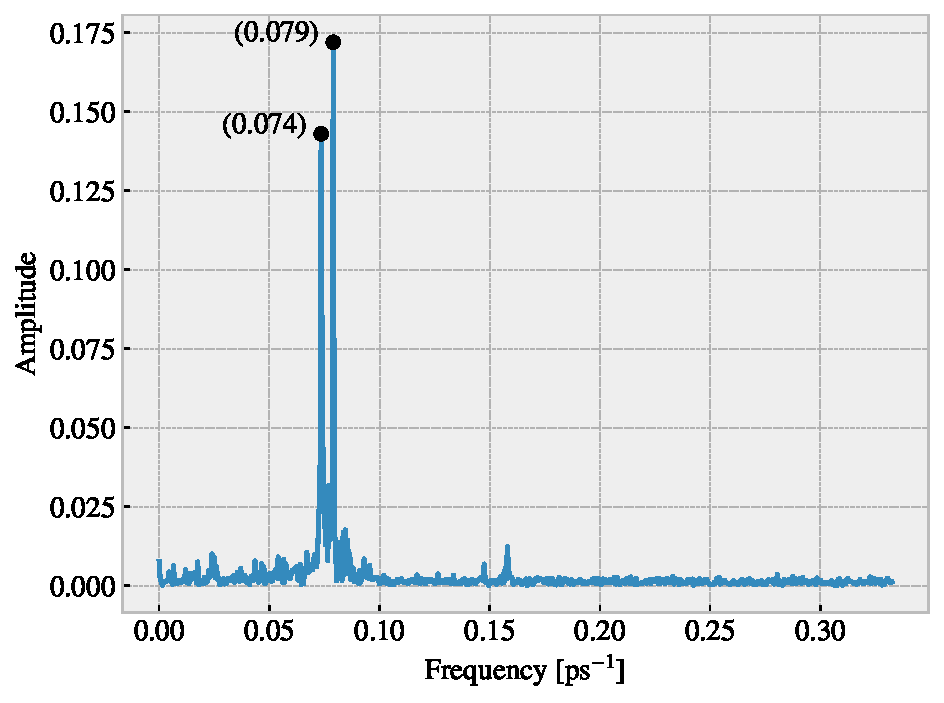
\includegraphics[width=\textwidth]{figures/baseline/ft_zoom.pdf}
    \caption{FT result shown for a reduced frequency range.}
    \label{fig:ft_a}
  \end{subfigure}
  \hfill
  \begin{subfigure}[t]{0.49\textwidth}
      \centering
      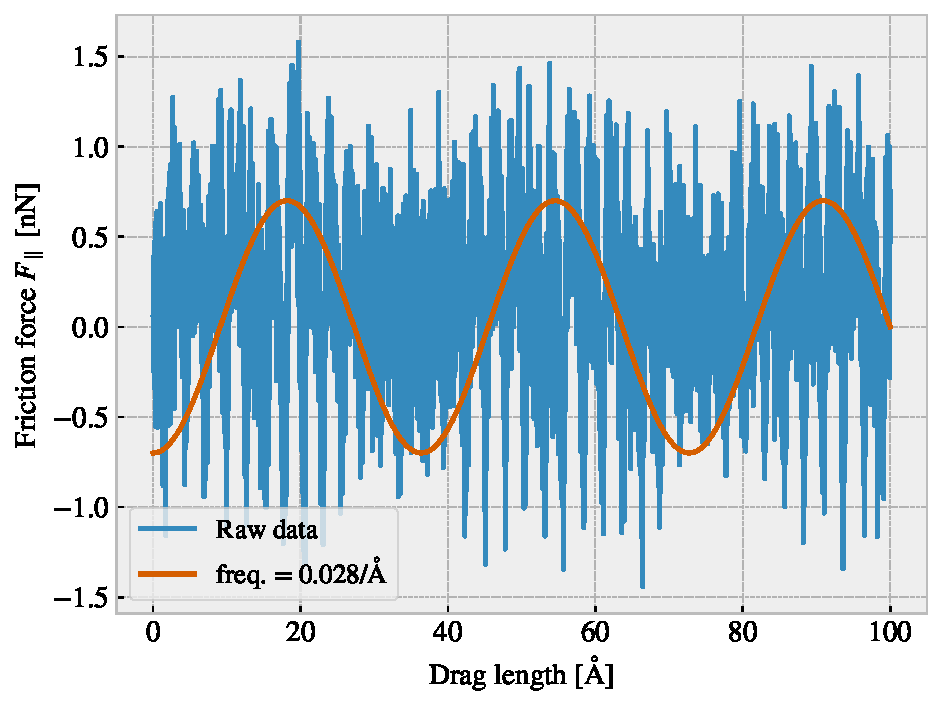
\includegraphics[width=\textwidth]{figures/baseline/ft_sine.pdf}
      \caption{Two most dominant frequencies applied to the data from \cref{fig:drag_Ff_100}}
      \label{fig:ft_b}
  \end{subfigure}
  \caption{Fourier transform analysis of the force traces shown in~\cref{fig:drag_Ff_10} and \cref{fig:drag_Ff_100}, but with the use of all \SI{400}{Å} of sliding. (a) The two most dominant frequency peaks from the Fourier analysis. Note that we cut off higher frequencies from the plot since no significant peaks were found there. (b) A comparison between the raw data and the wavefunction corresponding to the two peaks in panel (a).}
  \label{fig:ft}
\end{figure}


\subsection{Decompositions}
In the previous analysis, we considered the friction force acting on the entire
sheet, including the rigid pull blocks, and with respect to the sliding
direction. We found this way of measuring the friction force to be the most
intuitive and reliable, but we will present the underlying arguments for this
choice in the following.

Since we are only applying cuts to the inner sheet, and not the pull blocks, it
might appear more natural to only consider friction on the inner sheet. If the
desired frictional properties can be achieved by altering the inner sheet one
can argue that any opposing effects from the pull blocks can be mitigated by
simply adjusting the size ratio between the inner sheet and the pull blocks.
However, when looking at the force traces decomposed with respect to the inner
sheet and pull block regions respectively in~\cref{fig:decomp_group}, we observe
that the friction force arising from those parts is seemingly antisymmetric.
That is, the frictional force exerted by the substrate on the sheet oscillates
between the inner sheet and the pull blocks. Keeping in mind that normal force
is only applied to the pull blocks we might take this as an intrinsic feature of
the system that does not necessarily disappear with a scaling of the size ratio.
Any interesting friction properties might depend on this internal distribution
of forces. Hence, we hedge our bets and use the full sheet friction force as a
holistic approach to avoid excluding relevant features in the measurement data.

Similarly, we might question the decision of only considering the frictional
force projected onto the sliding direction as we are then neglecting the ``side
shift'' induced during sliding. In~\cref{fig:decomp_direc} we show the
decomposition in terms of the force components parallel $F_{\parallel}$ and
perpendicular $F_{\perp}$ to the sliding direction respectively. We notice that
the most dominant trend appears for the parallel component. One way to include
the perpendicular component is to evaluate friction as the length of the force
vector instead. However, this would remove the sign of the force direction and
shift the mean friction force up as we see both negative and positive
contributions in the parallel force trace. One option to accommodate this issue
is by using the vector length for the magnitude but keeping the sign from the
parallel component. However, we omit such compromises as this might make the
measurement interpretation unessercary complex, and we use only the parallel
component going forward. 

\begin{figure}[H]
  \centering
  \begin{subfigure}[t]{0.49\textwidth}
    \centering
    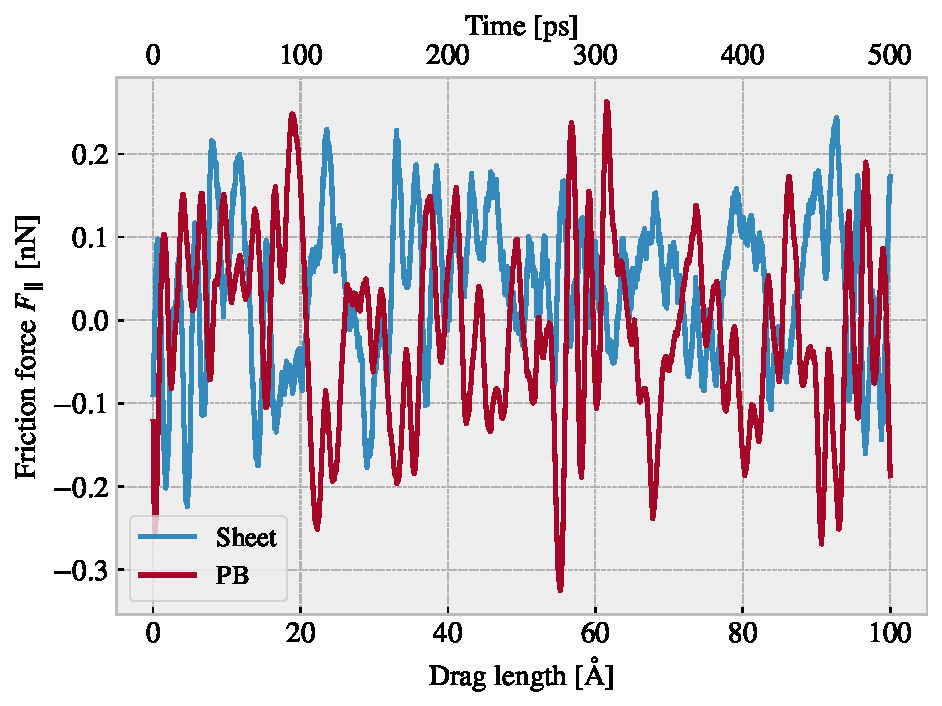
\includegraphics[width=\textwidth]{figures/baseline/decomp_group.pdf}
    \caption{}
    \label{fig:decomp_group}
  \end{subfigure}
  \hfill
  \begin{subfigure}[t]{0.49\textwidth}
      \centering
      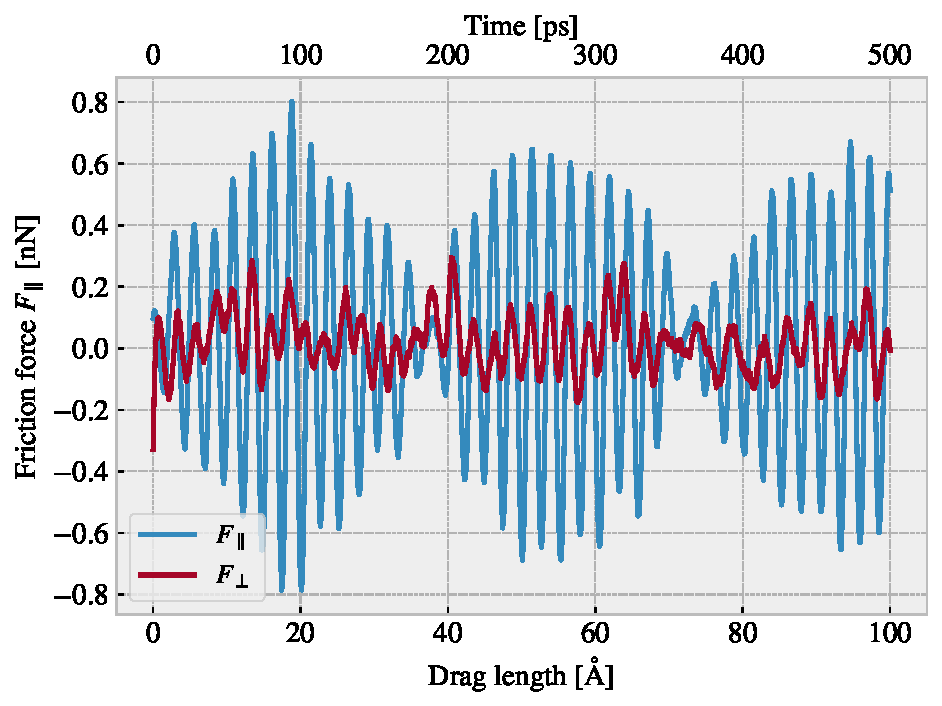
\includegraphics[width=\textwidth]{figures/baseline/decomp_direc.pdf}
      \caption{}
      \label{fig:decomp_direc}
  \end{subfigure}
  \caption{Friction force decomposition on the default parameter force trace shown in~\cref{fig:drag_Ff}. We show only the Savgol filters here. (a) Decomposition into the sheet regions inner sheet (sheet) and pull blocks (PB). (b) Decomposition into friction force parallel ($F_{\parallel}$) and perpendicular ($F_{\perp})$ to the sliding direction.}
  \label{fig:decomp}
\end{figure}


\subsection{Center of mass path}
From the previous observations of the force traces in~\cref{fig:drag_Ff} we found both smooth sliding and stick-slip behavior depending on the sliding speed and spring constant. Considering the force
decomposition in~\cref{fig:decomp_direc} we know that a frictional force in
the perpendicular direction to sliding is also present. By looking at the
$x,y$-position for the sheet Center of Mass (\acrshort{CM}) we find a qualitatively different behavior when reconsidering the spring constants and sliding speeds investigated in~\cref{fig:drag_Ff}. These results are shown in~\cref{fig:CM_path}. The default case in~\cref{fig:CM_path_def} shows a rather straight path with
only a small side motion in comparison to the cases in~\cref{fig:CM_path_K10_v10} and~\cref{fig:CM_path_K10_v1}. However, the \acrshort{CM} accelerates and deaccelerates with a high frequency, much too high
to be associated with the lattice spacing on the order of \SI{2.46}{Å}. One possible explanation is that the sheet and substrate
constitute an incommensurable contact for which traveling kink excitations make
the atoms move in such a way that the sheet \acrshort{CM} is incremented in small ``bursts''. When looking at the $K = \SI{10}{\frac{N}{m}}$, $v =
\SI{10}{\frac{m}{s}}$ case in~\cref{fig:CM_path_K10_v10} we see a completely
different \acrshort{CM} path where the rapid movements align visually better with
the force oscillations shown earlier in \cref{fig:drag_Ff_100_K10_v10}. The
\acrshort{CM} accelerates forward and then deaccelerates in combination with a
side motion that leads to the \acrshort{CM} path making a loop as it slows down.
Finally we have the $K = \SI{10}{\frac{N}{m}}$, $v = \SI{10}{\frac{m}{s}}$ in~\cref{fig:CM_path_K10_v10} which is confirmed to have stick-slip behavior in~\cref{fig:drag_Ff_100_K10_v1}. Here the \acrshort{CM} path shows a more chaotic
movement between accelerations, but with the rapid parts aligning visually well with the timing of the slips seen in~\cref{fig:drag_Ff_100_K10_v1}. We might associate the chaotic motion with thermal contributions as these are thought to be dominant at lower sliding speeds.  


\begin{figure}[H]
  \centering
  \begin{subfigure}[t]{0.85\textwidth}
    \centering
    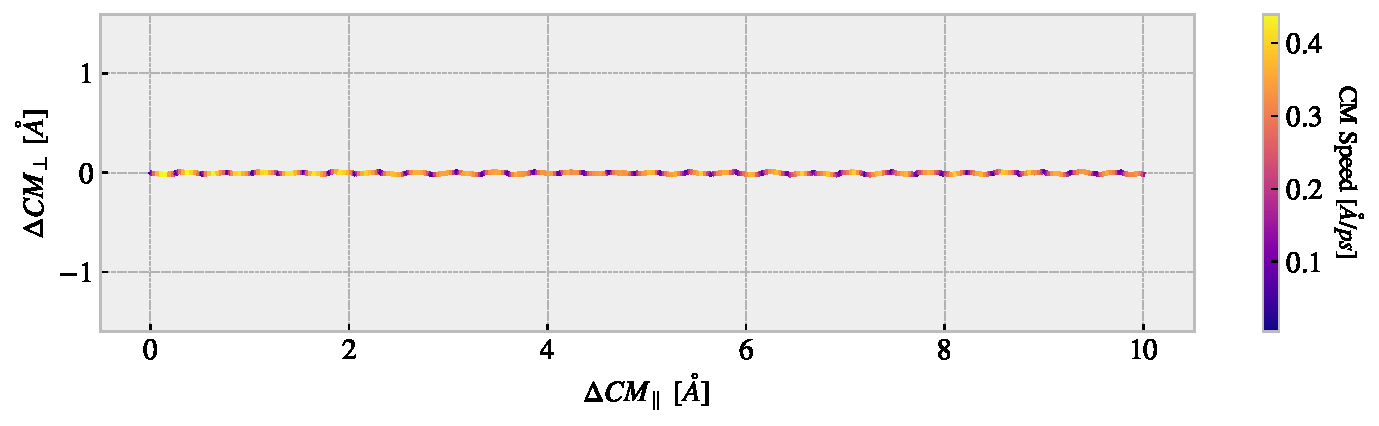
\includegraphics[width=\textwidth]{figures/baseline/COM_path_K0.pdf}
    \caption{$K = \inf$, $v = \SI{20}{\frac{m}{s}}$.}
    \label{fig:CM_path_def}
  \end{subfigure}
  \hfill
  \begin{subfigure}[t]{0.85\textwidth}
    \centering
    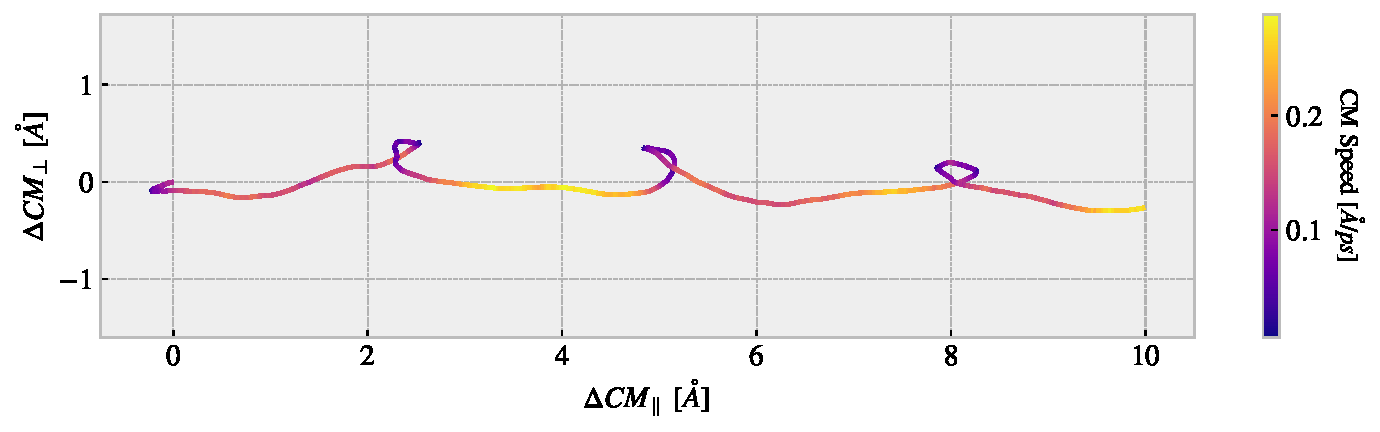
\includegraphics[width=\textwidth]{figures/baseline/COM_path_K10_v10.pdf}
    \caption{$K = \SI{10}{\frac{N}{m}}$, $v = \SI{10}{\frac{m}{s}}$.}
    \label{fig:CM_path_K10_v10}
  \end{subfigure}
  \begin{subfigure}[t]{0.85\textwidth}
    \centering
    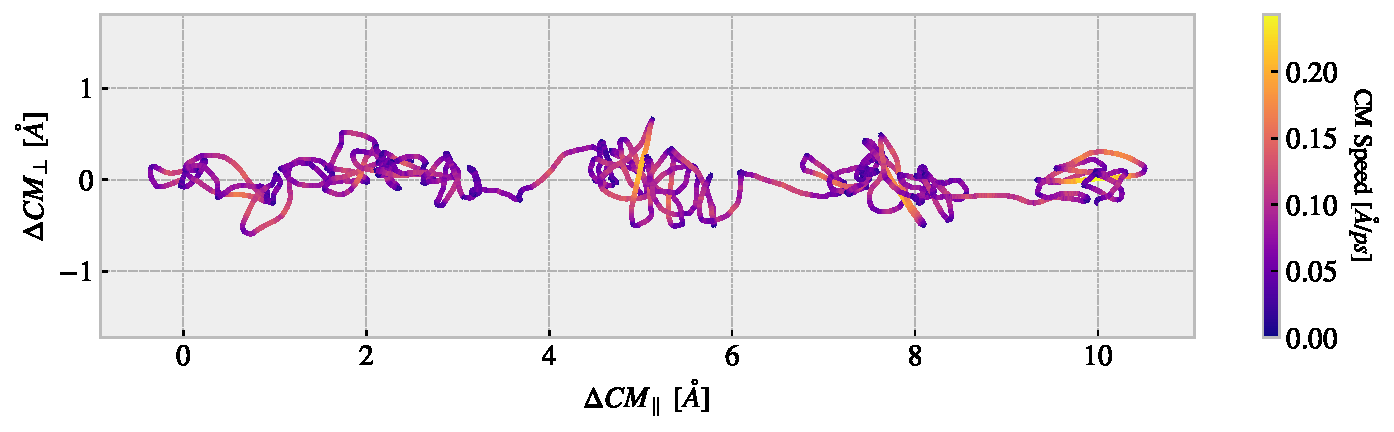
\includegraphics[width=\textwidth]{figures/baseline/COM_path_K10_v1.pdf}
    \caption{$K = \SI{10}{\frac{N}{m}}$, $v = \SI{1}{\frac{m}{s}}$.}
    \label{fig:CM_path_K10_v1}
  \end{subfigure}
  \caption{Sheet Center of Mass (\acrshort{CM}) position relative to the start of the sliding phase in terms of the direction parallel to the sliding direction $\Delta COM_{\parallel}$ and the axis perpendicular to the sliding direction $\Delta COM_{\perp}$. The colors denote the absolute speed of the \acrshort{CM} motion. Figure (a)-(c) shows different parameters used for the spring constant $K$ and sliding speed $v$ similar to that used in~\cref{fig:drag_Ff}. (a) Default: $K = \inf$, $v = \SI{20}{\frac{m}{s}}$. (b) Values adopted from Zhu
  and Li~\cite{zhu_study_2018}: $K = \SI{10}{\frac{N}{m}}$, $v = \SI{10}{\frac{m}{s}}$. (c) $K = \SI{10}{\frac{N}{m}}$, $v = \SI{1}{\frac{m}{s}}$ }
  \label{fig:CM_path}
\end{figure}


\section{Defining metrics for friction}\label{sec:fric_metrics}
In order to evaluate the frictional properties of the sheet we aim to reduce the force trace results, addressed in~\cref{sec:single_analysis}, into single metrics describing the kinetic and static friction respectively. 

\subsection{Kinetic friction}
We measure kinetic friction as the mean of the friction force trace. More
precisely, we take the mean value of the last half of the dataset in order to
ensure that we are sampling from a stable system. For a full sliding simulation
of \SI{400}{\text{Å}} our mean value will be founded on the last
\SI{200}{\text{Å}} (\SI{1000}{ps}) of sliding. In~\cref{fig:runmean} we have
shown the force trace for the first \SI{10}{\text{Å}} of sliding together with a
50\% running mean window. The choice of such a short sliding distance is merely
to illustrate the sampling procedure, and we see that the final mean estimate
(marked with a dot) takes a negative value due to the specific cut-off of the
few oscillations captured here. Nonetheless, one approach to quantifying the
uncertainty of the final mean estimate is to consider the variation of the
running mean preceding the final mean value. The more the running mean
fluctuates the more uncertainty associated with the final estimate. Only the
running mean ``close'' to the ending should be considered, since the first part
will rely on data from the beginning of the simulation. From the Fourier analysis
in~\cref{sec:force_oscillations} we found the longest significant
oscillation period to be $\sim \SI{71}{\text{Å}}$. Hence, we find it reasonable
to use the standard deviation (\acrshort{std}) for the last $\sim
\SI{71}{\text{Å}}$ of the running mean window to evaluate the fluctuations. When
including the full sliding length this corresponds to the last $\sim 35 \%$ of
the running mean window ($\SI{400}{\text{Å}}\cdot 50\% \cdot 35\% \approx \SI{71}{\text{Å}}$). We consider the \acrshort{std} as an estimate of the
absolute error and calculate the relative error by a division of the final mean
value. In~\cref{fig:runstd} we showcase a running relative error based on the
\acrshort{std}, with a window of length 35\% the mean window, in a continuation
of the illustrative case of a \SI{10}{\text{Å}} sliding from~\cref{fig:runmean}.
In this case, we get an extremely high relative error of $\sim 257\%$, but this
is consistent with the fact that the short sampling period leads to an
unphysical negative value which should be associated with high uncertainty. 

\begin{figure}[H]
  \centering
  \begin{subfigure}[t]{0.49\textwidth}
    \centering
    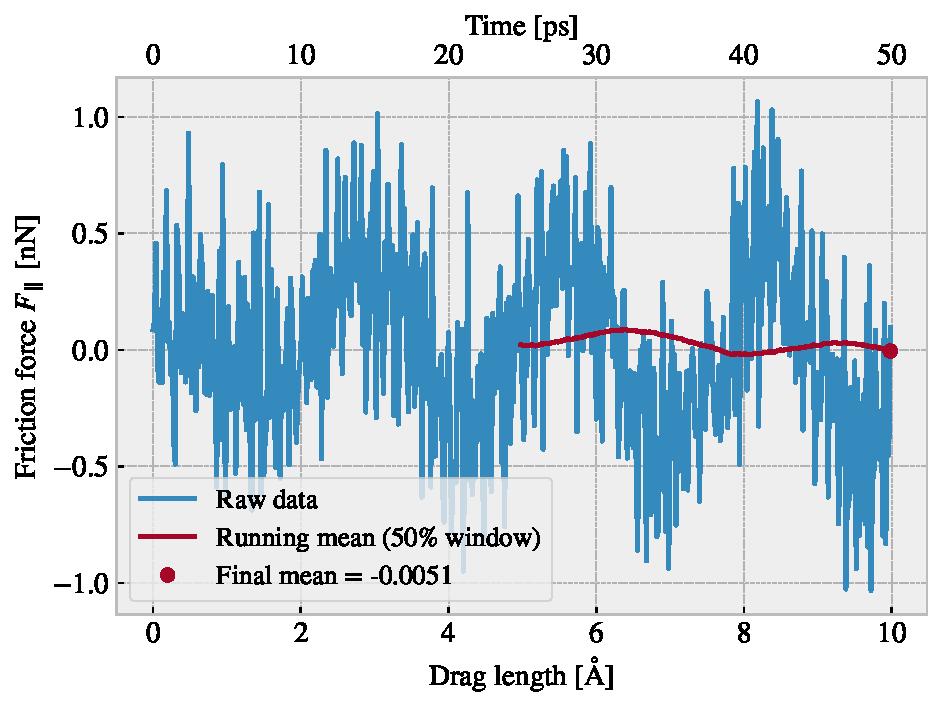
\includegraphics[width=\textwidth]{figures/baseline/Ff_runmean.pdf}
    % \caption{Running mean with window length $\SI{5}{\text{Å}}$ (50\% the data length).}
    \caption{}
    \label{fig:runmean}
  \end{subfigure}
  \hfill
  \begin{subfigure}[t]{0.49\textwidth}
      \centering
      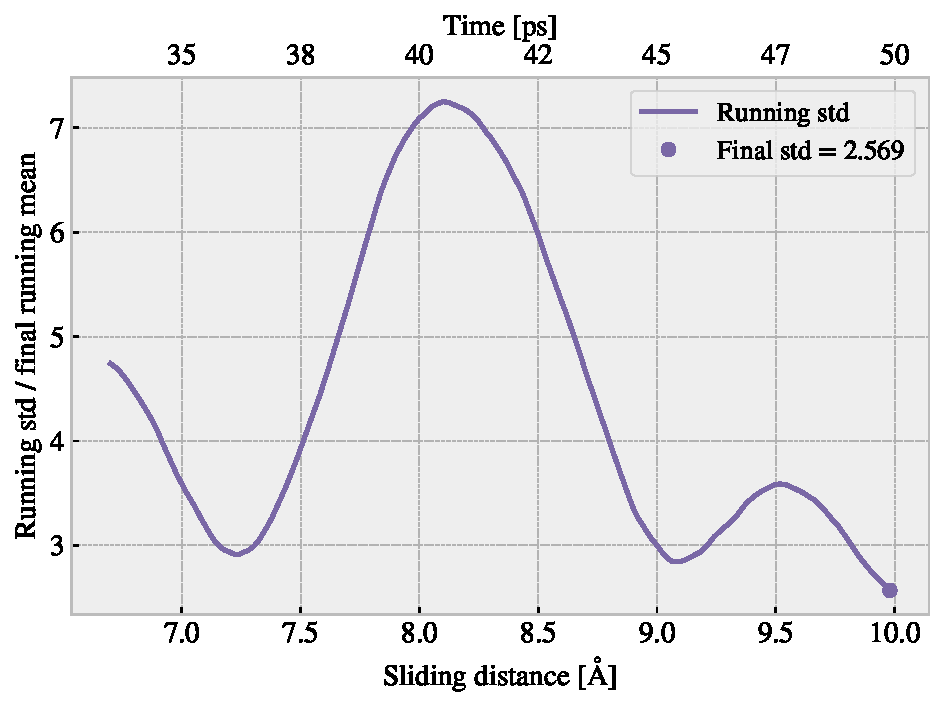
\includegraphics[width=\textwidth]{figures/baseline/Ff_runstd.pdf}
      \caption{}
      \label{fig:runstd}
  \end{subfigure}
  \caption{Supporting figures for the description of the kinetic friction metric and corresponding uncertainty for an example using a reduced sliding distance of \SI{10}{{\text{Å}}}. (a) The running mean for the force trace with a window length of 50\% of the sliding length in this example. (b) The running relative error calculated using the standard deviation for the 35\% running window of the running mean (red line) in panel (a). For both figures, the running value is displayed at the end of their respective corresponding windows.}
  \label{fig:running}
\end{figure}

When including the full dataset of \SI{400}{\text{Å}} of sliding, such that the \acrshort{std} window actually matches with the longest period of oscillations expected, we get a final relative error of $\sim 12 \%$ as shown in fig~\cref{fig:runstd_long}. This is arguable just at the limit of an acceptable error, but as we shall see later on in~\cref{sec:load_and_stretch} this high relative error is mainly associated with the cases of low friction. When investigating different configurations under variation of load and strain we see a considerably lower relative error as the mean friction evaluates to higher values. One interpretation of this finding is that the oscillations in the running mean are not substantially influenced by the magnitude of the friction. In that case, the relative error will spike for the low friction cases, and the absolute error might be the more reliable measure, i.e.\ using simply the \acrshort{std} without dividing by the final mean value.


\begin{figure}[H]
  \centering
  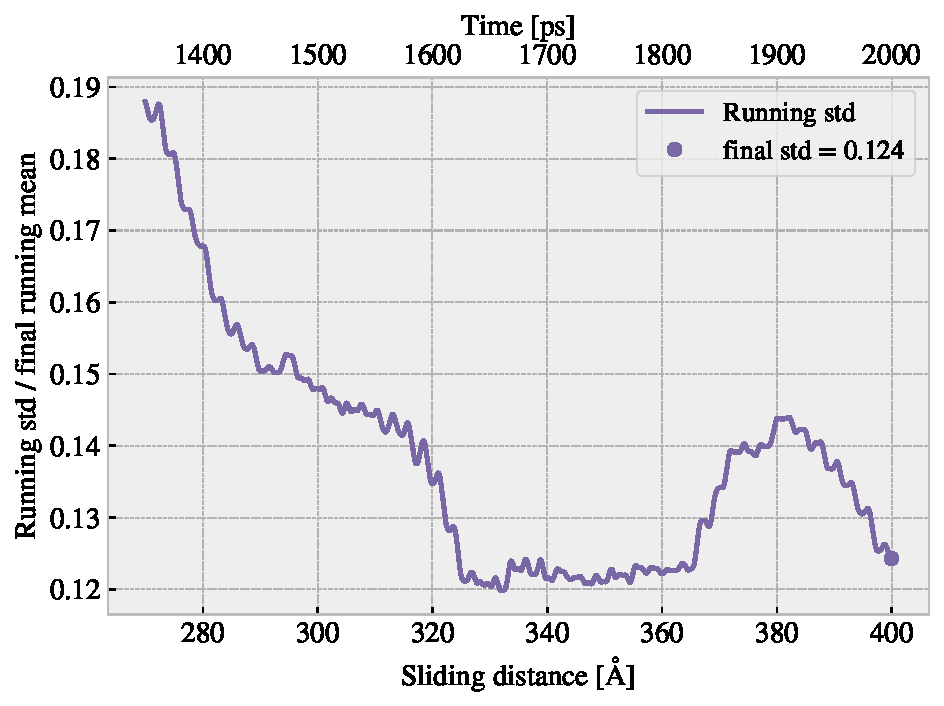
\includegraphics[width=0.6\linewidth]{figures/baseline/Ff_runstd_long.pdf}
  \caption{Running standard deviation (std) for a full \SI{400}{{\text{Å}}} sliding simulation. The running std window is \SI{70}{\text{Å}} (35\% of the running mean window, which is 50\% of the full sliding length).}
  \label{fig:runstd_long}
\end{figure}


\subsection{Static friction} 
The maximum value is one of the common choices for addressing static friction,
even though the definition of static friction is a bit vague. When considering
the force traces in~\cref{fig:drag_Ff} we observe that the force oscillations
increase in magnitude toward a global peak at $\sim \SI{20}{\text{Å}}$. Thus,
one could be inclined to identify this peak as the maximum value associated with
the static friction force. However, as we have already clarified, this steady
increase in friction is part of a slower oscillation that repeats with a period
of $\sim \SI{71}{\text{Å}}$. By plotting the top three max values recorded
during a full \SI{400}{Å} simulation, for 30 logarithmically spaced load values
in the range $[0.1, 100]$ nN, we observe that the global max rarely falls within
this first oscillation period as shown in~\cref{fig:max_dist}. Only 2 out of 30
global maxima and 4 out of 90 top three maxima can be associated with the start
of the sliding by this definition. Thus, this result suggests that our default
system does not yield a static friction response in the sense of an initial
increase in friction due to a depinning of the sheet from the static state.
Several modifications to the system parameters may enhance the likelihood of
observing a substantial static friction response. These include prolonging the
initial relaxation time, as static friction is believed to increase
logarithmically with time~\cite{dieterich_1972}, or increasing the sliding force
more slowly by utilizing a soft spring tethering. As an attempt to test the
latter part of this hypothesis, we conducted a series of simulations with
different spring constants, $K\in [5, 200]$ nN, including also $K = \infty$,
while maintaining the relaxation period and sliding velocity at their default
values. The results shown in~\ref{fig:max_vs_K} do not support this hypothesis
since the reduction of the spring constant did not lead to the maximum
friction peak appearing within the first oscillation period. We acknowledge that
this outcome might be compromised by our choice of the relaxation period or sliding speed. However, given the
ambiguity surrounding the determination of static friction, we will mainly
concern ourselves with kinetic friction in the remainder of this thesis.


% In most numerical studies \cite{bonelli_atomistic_2009, zhu_study_2018} they define static friction as the max peak or top 5\% quantile throughout the simulation and do not consern themselves with a requirement for an initial increasement toward this max. Thus, we interpret this as a measure of the force oscillation magnitude which is highly related to the stick-slip behaviour. 


\begin{figure}[H]
  \centering
  \begin{subfigure}[t]{0.49\textwidth}
      \centering
      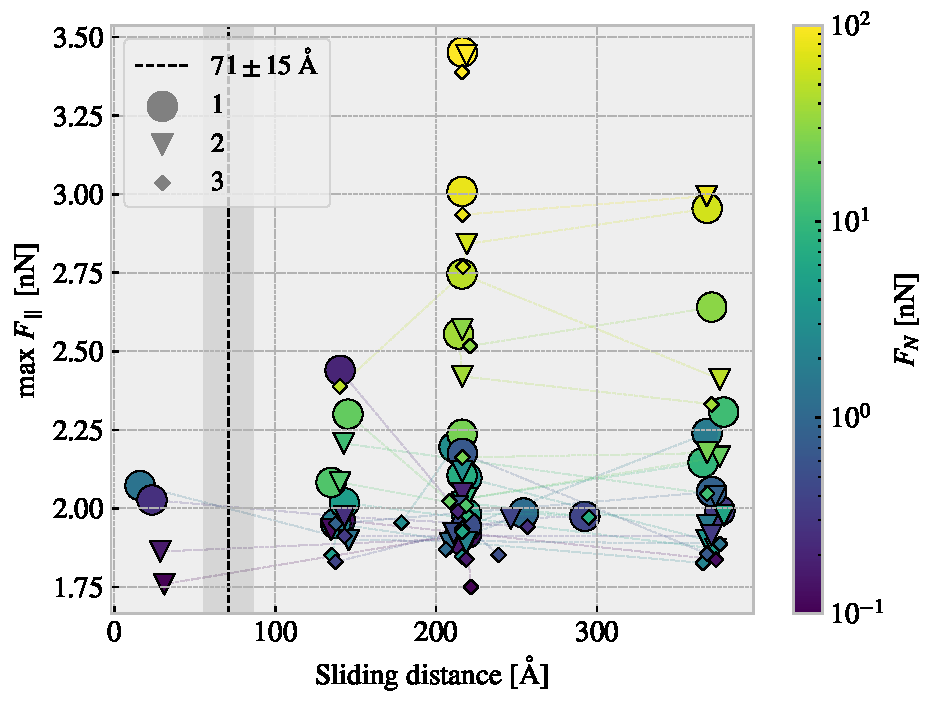
\includegraphics[width=\textwidth]{figures/baseline/max_dist.pdf}
      \caption{}
        \label{fig:max_dist}
    \end{subfigure}
    \hfill
    \begin{subfigure}[t]{0.49\textwidth}
      \centering
      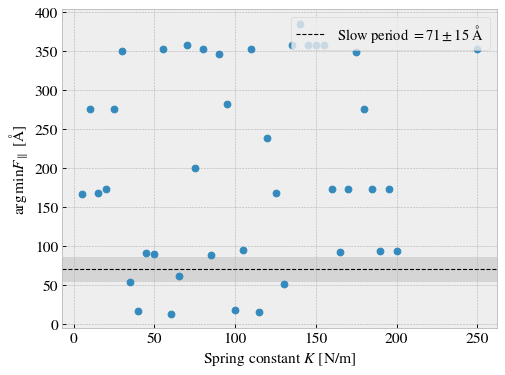
\includegraphics[width=\textwidth]{figures/baseline/max_vs_K}
      \caption{}
      \label{fig:max_vs_K}
    \end{subfigure}
    \caption{Investigation of the sliding displacement corresponding to the maximum friction force peaks. The dotted line, along with the gray-shaded area indicating the degree of uncertainty, represents the slowest significant oscillation period identified in the data. This line serves as a threshold for determining whether a peak falls within the initial portion of the sliding simulation. (a) The top three maxima for simulations with varying loads; 30 logarithmically spaced loads in the range $[0.1, 100]$ nN. The marker shapes denote the top 1, 2 and 3 respectively and the color denotes the normal load. (b) The sliding displacement corresponding to the friction maxima for simulations with varying spring constant; 40 uniformly spaced values in the range $K \in [5, 200]$ N/m in addition to $K = \infty$.}
    \label{fig:max_peaks}
\end{figure}


% \begin{figure}[H]
%   \centering
%   \begin{minipage}{.47\textwidth}
%     \centering
%     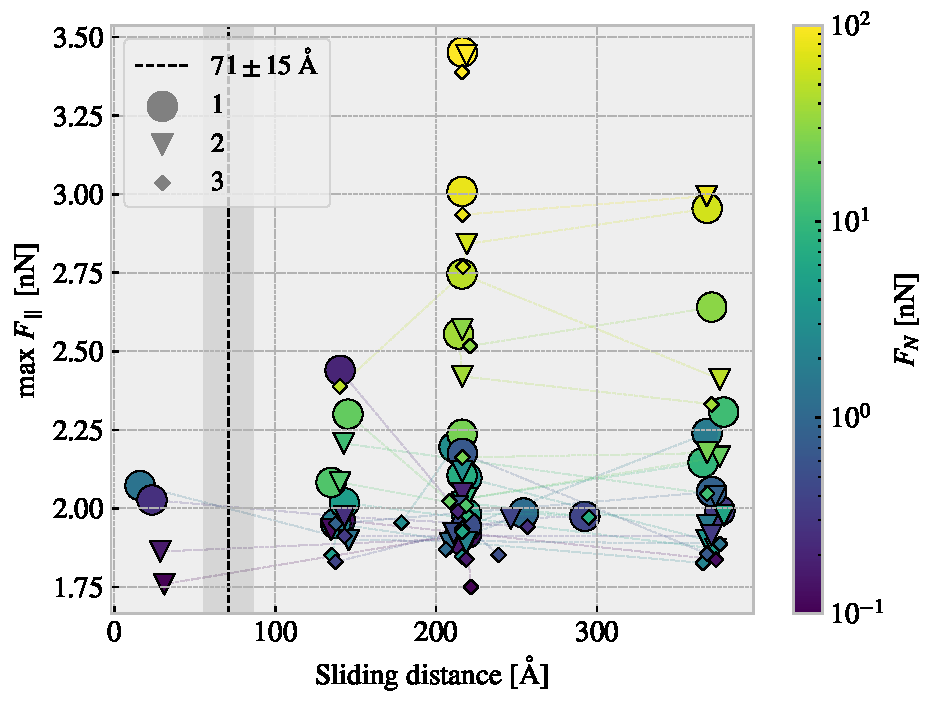
\includegraphics[width=\linewidth]{figures/baseline/max_dist.pdf}
%     \captionof{figure}{The distribution of the top three maximum friction force peaks resulting from multiple friction simulations with varying loads, for 30 logarithmically spaced load values in the range $[0.1, 100]$ nN. The dotted line, along with the gray-shaded area indicating the degree of uncertainty, represents the slowest significant oscillation period identified in the data. This line serves as a threshold for determining whether a peak falls within the initial portion of the sliding simulation.}
%     \label{fig:max_dist}
%   \end{minipage}%
%   \hspace{0.2cm}
%   \begin{minipage}{.48\textwidth}
%     \centering
%     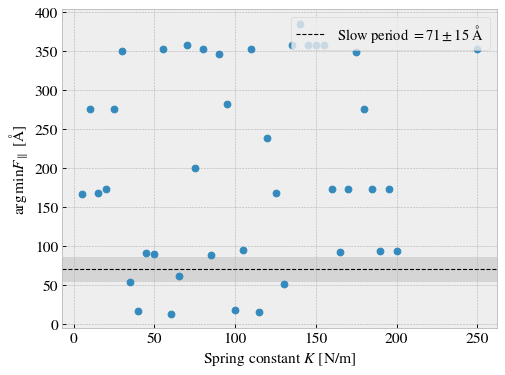
\includegraphics[width=\linewidth]{figures/baseline/max_vs_K}
%     \captionof{figure}{Sliding displacement corresponding to the maximum friction force as a function of spring constant.}
%     \label{fig:max_vs_K}
%   \end{minipage}
%   \end{figure}





% We investigate the placement of the max values, i.e. the sliding distance length for which we measure the max friction force. We show the placement of the top three max values for different simulatiosn with varying normal force in \cref{fig:max_dist}. We observe immediately that only a few top three max values is measured within a full slow period of $\sim$ 71 Å. In fact many max values is measured just before the end of the simulation. This indicates that the naive approach of using the overall max value to describe the static friction coefficient might be a to naive approach. Another approach is to use the max value within a single period, but we do not really know if this period will be similar for alle cut patterns and thus this might be limiting. 



% Look into static friction when having a spring connected to the drag force with
% rather low spring constant. Maybe compare to critical sitffness in FK model.
% Some rough calculations follow here (make a note about this being a very naive
% approach to determine a suitable stiffness for static friction scenarious. In
% reality one should increase force slowly to observe this probably). When
% dragging the sheet in the y-direction we effectively have a lattice spacing
% \begin{align*}
%   a_c = a_{2,x} + B_x = a_G\frac{\sqrt{3}}{2} + \frac{a_G}{2\sqrt{3}} = \frac{2a_G}{\sqrt{3}}
% \end{align*}
% for graphene lattice constant $a_G = 2.46$ Å. For the diamond silicon structure
% this is essentially equal to the lattice constant $a_D = 5.4210$ Å. This gives 
% \begin{align*}
%   \theta = \frac{a_c}{a_b} = \frac{2}{\sqrt{3}}\frac{a_G}{a_D} \approx 0.5230.
% \end{align*}
% Since we have the factor $2/\sqrt{3}$ it is safe to assume that this is a
% irrational number leadning to incommensurability. The worst case scnario of
% incommensurability (where $\theta$ equals the golden-mean, Can we get the exact
% number?) gives the minimal critical stiffness $K_c \sim 2U_0
% (\frac{\pi}{a_b})^2$, where $U_0$ is the substrate potentiual magnitude and
% $a_b$ the lattice spacing of the substrate. The potential barrier $U_0$ can be
% approximated by the work done when resisting the normal force as $\sim F_N
% a_D/2$ such that the critical stiffness can be approximated to 
% \begin{align*}
%   K_c \sim 2 F_N \frac{a_D}{2} \left(\frac{\pi}{a_D}\right)^2 = \frac{F_N}{a_D}\pi^2
% \end{align*}
% With a normal force of 1 nN we get $K_c \sim 18$ N/m. Hence, we should try a
% spring constant lower than that as qualified way of determining if this is the
% reason why we do not really see static friciton in the simulation. By plotting the max position (in terms of drag length) as a function of spring constant as seen in \cref{fig:max_vs_K} we can investigate if the concept of a critical spring constant is governing this simulation. However, as I'm writing this I'm realizing that the spring constant in the model applies to the interatomic forces and not the one dragging the system.....




\section{Out-of-plane buckling}\label{sec:out-of-plane_buckling}
The out-of-plane buckling is one of the motivations for investigating
the application of Kirigami cuts in the context of friction properties. Therefore, we perform a stretch simulation, at low temperature ($T = \SI{5}{K}$) without any substrate, in order to verify that we can reproduce an out-of-plane buckling with the Tetrahedron and Honeycomb patterns. For this investigation, we consider the Tetrahedron $(7,5,1)$ and the Honeycomb $(2,2,1,5)$ pattern in comparison to the non-cut sheet. We quantify the out-of-plane buckling by assessing the distribution of atoms along the z-direction (perpendicular to the plane) during straining. We calculate the
minimum and maximum z-value as well as the atom count quartiles 1\%, 10\%, 25\%, 50\% (median), 75\%, 90\% and 99\% as shown in~\cref{fig:buckling_quartiles}. The Tetrahedron and Honeycomb patterns show significant buckling in comparison to the non-cut sheet, which only exhibits minor buckling of $\sim \SI{2}{\text{Å}}$, which is of the same order as the lattice spacing. We notice that the Tetrahedron pattern buckles more in consideration to the min.\ and max.\ peaks while the remaining quantiles seem to be more closely spaced than for the Honeycomb. By addressing the simulation results visually, using the \textit{Open Visualization Tool OVITO}, we find that this can be attributed to fringes on the edge ``flapping around'' and thus increasing the min.\ and max.\ values. This is also evident from the simulation with the substrate seen in \cref{fig:tetrahedron_strain_j} in~\cref{sec:sheet_stretch}.

\begin{figure}[H]
  \centering
  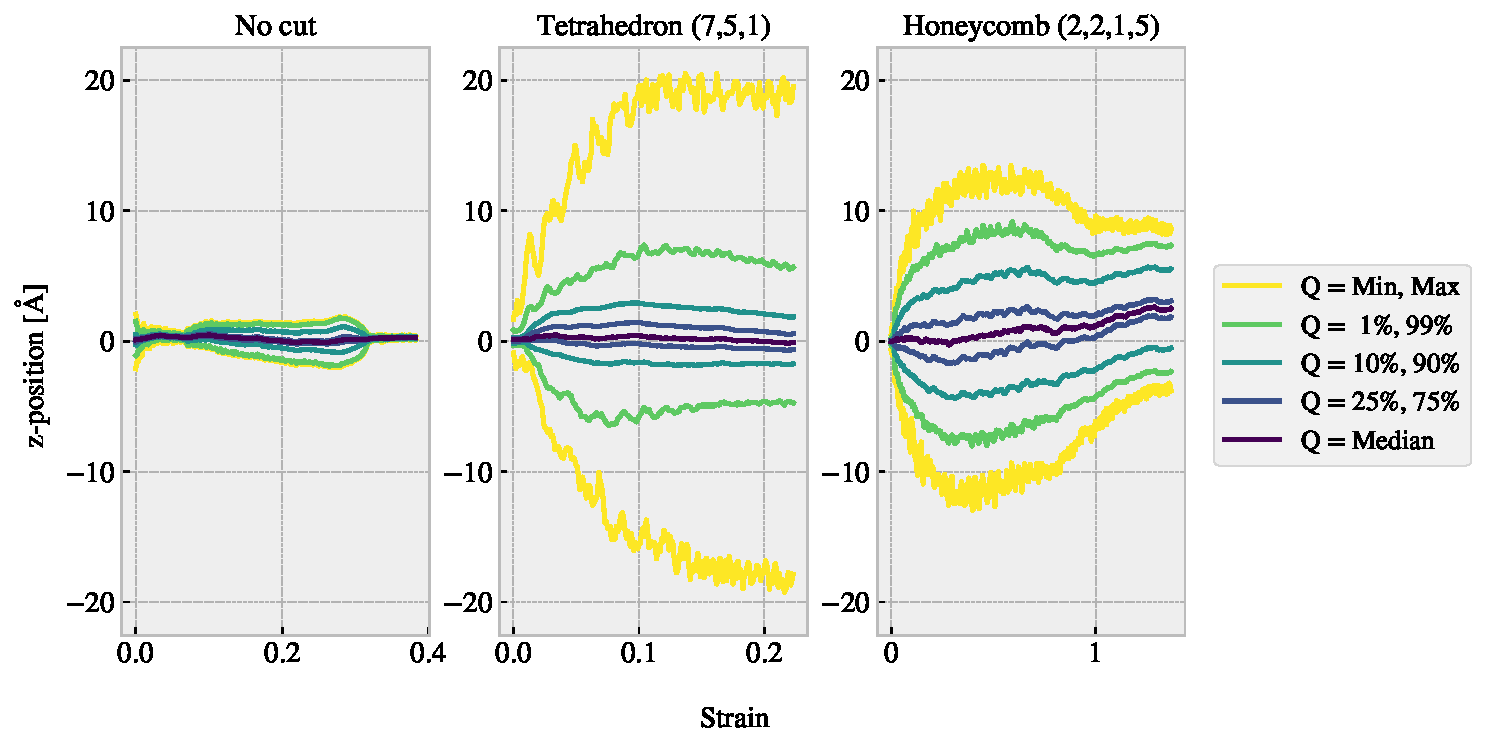
\includegraphics[width=\linewidth]{figures/baseline/vacuum_normal_buckling.pdf}
  \caption{The out-of-plane buckling during straining for three different sheet patterns, namely the No cut, Tetrahedron $(7,5,1)$, and Honeycomb $(2,2,1,5)$ pattern, in vacuum at low temperature $T = \SI{5}{K}$. The buckling is quantified by the distribution of the atom z-positions, which are perpendicular to the sheet plane, and the colors indicate selected quantiles. The yield strain for each pattern, from left to right, is 0.38, 0.22, and 1.37, respectively. The results indicate that the Tetrahedron and Honeycomb patterns exhibit significantly out-of-plane buckling in comparison to the non-cut sheet.}
  \label{fig:buckling_quartiles}
\end{figure}

Given the confirmation of out-of-plane buckling in a vacuum, as seen
in~\cref{fig:buckling_quartiles}, we reintroduce the substrate in order to
investigate whether this effect carries over to a changing contact area. For
this simulation, we raise the temperature to the default value of $T
=\SI{300}{K}$. We keep the normal force off and let the sheet stick purely by
the adhesion forces between the sheet and substrate. We quantify the contact
area through the relative number of atoms in the sheet within chemical range of
the substrate. The cut-off for this interaction is set to 4 Å, adopted
from~\cite{li_evolving_2016}, corresponding to $\sim 120\%$ the \acrshort{LJ}
equilibrium distance. Usually, the contact area is calculated as the number of
contacting atoms multiplied by an associated area for each atom. However, since
we are not interested in the absolute value of the area, but rather the relative
change, we omit the multiplication factor. That is, we consider the relative
number of atoms within the contact range as our metric of choice, which is
proportional to the contact area. The relative contact for the three
configurations (No cut, Tetrahedron $(7,5,1)$ and Honeycomb $(2,2,1,5)$) during
straining are shown in~\cref{fig:contact_vs_stretch}. The figure reveals
a significant drop in relative contact as the sheets are strained, which agrees
qualitatively with the buckling observed in~\cref{fig:buckling_quartiles}
without the substrate. The Honeycomb pattern turned out to be both the most
stretchable, with a rupture strain of 1.27, and the one with the biggest
decrease in relative contact with a minimum of approximately 43\%. Notice, that
the relative contact is never actual 1.0 but instead reaches a maximum of 96\%
without strain. This is attributed to the temperature fluctuations and the
choice of cut-off. 

Selected frames from the simulation result are shown in~\cref{sec:sheet_stretch}
which reveals a bit more information on how the buckling occurs. The Tetrahedron pattern deforms rather quickly and smoothly into small tetrahedron
spikes, as the name suggests. In the Honeycomb pattern, on the other hand, the
deformations initiate from one side first. As the sheet stretches more rows of
the pattern are activated, producing the honeycomb-looking shape when seen from
above. Both patterns exhibit a small increase in relative contact when they
are approaching their yield strain, which agrees with the results from ~\cref{fig:buckling_quartiles} where the buckling reduces slightly towards the
rupture strain.


\begin{figure}[H]
  \centering
  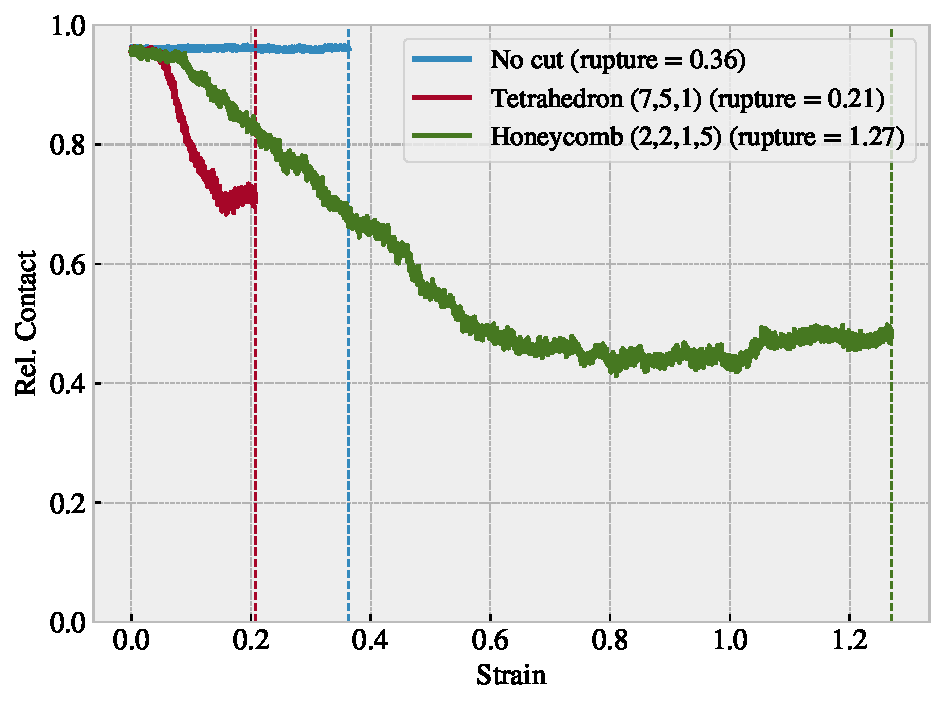
\includegraphics[width=0.6\linewidth]{figures/baseline/contact_vs_stretch.pdf}
  \caption{Relative contact, given as the relative number of atoms in the sheet being within chemical interaction range, vs.\ straining of the sheet. The cut-off for the interaction range is \SI{4}{\text{Å}} corresponding to $\sim 120 \%$ the \acrshort{LJ} equilibrium distance. No normal force is applied and temperature is kept at $T = \SI{300}{K}$.}
  \label{fig:contact_vs_stretch}
\end{figure}




\section{Investigating default parameters}\label{sec:main_params}
We carry out a more extensive investigation of the friction dependence on temperature $T$, sliding speed $v_{\text{slide}}$, spring
constant $K$, and timestep $dt$. This is done partly to
understand how the dependencies relate to the theoretical, numerical and
experimental results, and partly to understand how these parameters affect
the stability of our system. We use the default parameters presented in~\cref{tab:final_param} and investigate the results as we change parameters, one at a time. We keep the load at \SI{1}{nN}. We consider the mean
friction force, sampled from the last half of the simulation as described in~\cref{sec:fric_metrics}, representing the kinetic friction. The results are shown in~\cref{fig:main_param}, where the shaded area (connected linearly) denotes the absolute error defined by the \acrshort{std} as described in~\cref{sec:fric_metrics} as well. 

\begin{figure}[H]
  \centering
  \begin{subfigure}[t]{0.49\textwidth}
      \centering
      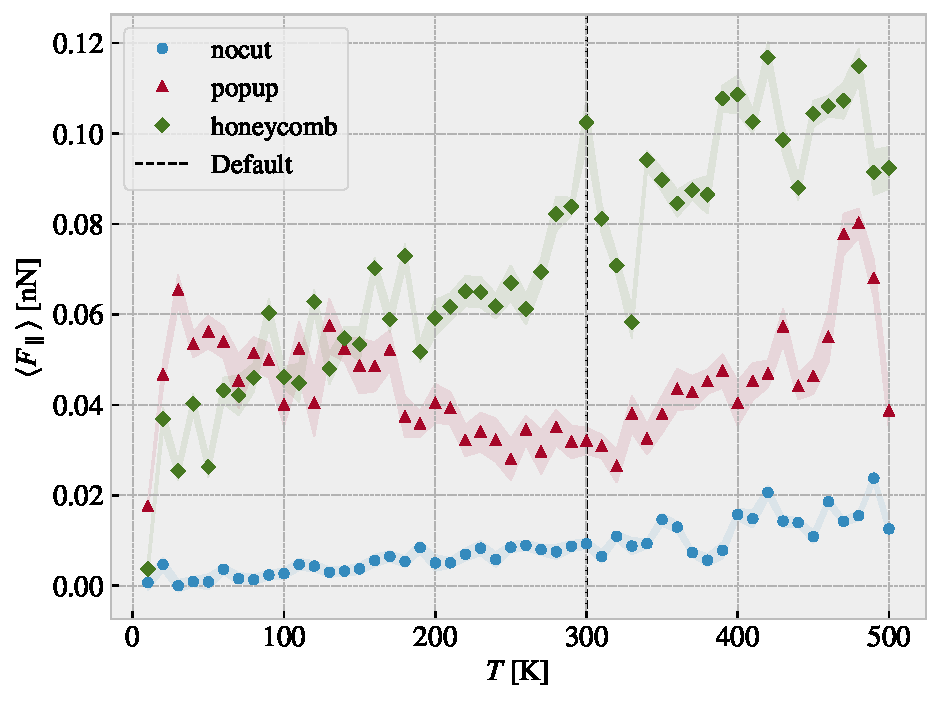
\includegraphics[width=\textwidth]{figures/baseline/variables_temp_mean_fixmove_v20.pdf}
      \caption{}
      \label{fig:var_temp}
    \end{subfigure}
    \hfill
    \begin{subfigure}[t]{0.49\textwidth}
      \centering
      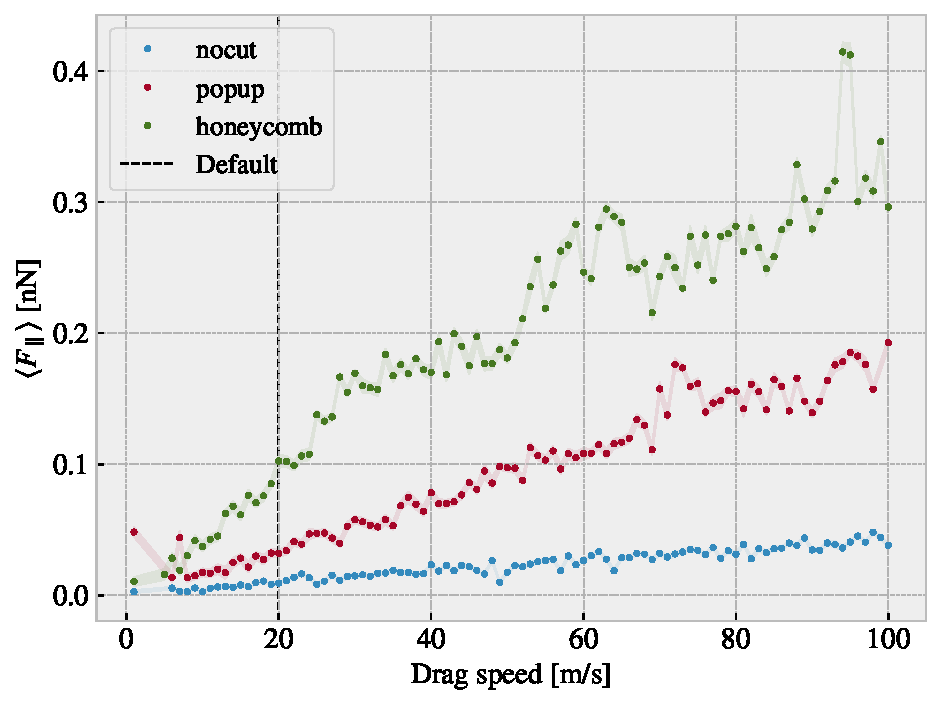
\includegraphics[width=\textwidth]{figures/baseline/variables_vel_mean_fixmove.pdf}
      \caption{}
      \label{fig:var_vel}
    \end{subfigure}
    \hfill
    \begin{subfigure}[t]{0.49\textwidth}
      \centering
      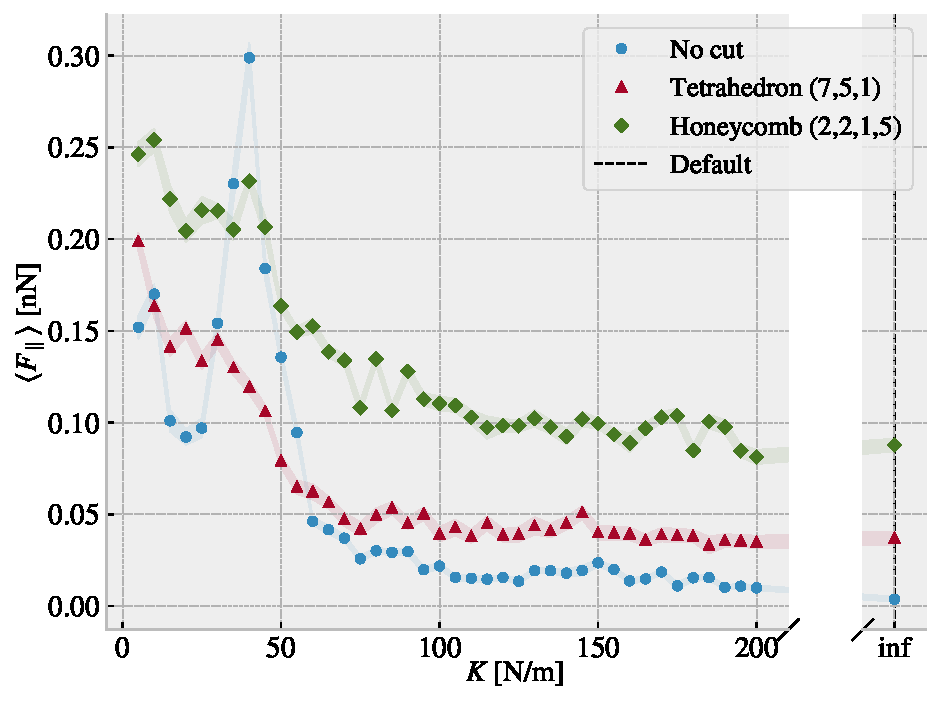
\includegraphics[width=\textwidth]{figures/baseline/variables_spring_mean_fixmove.pdf}
      \caption{}
      \label{fig:var_K}
    \end{subfigure}
    \hfill
    \begin{subfigure}[t]{0.49\textwidth}
        \centering
        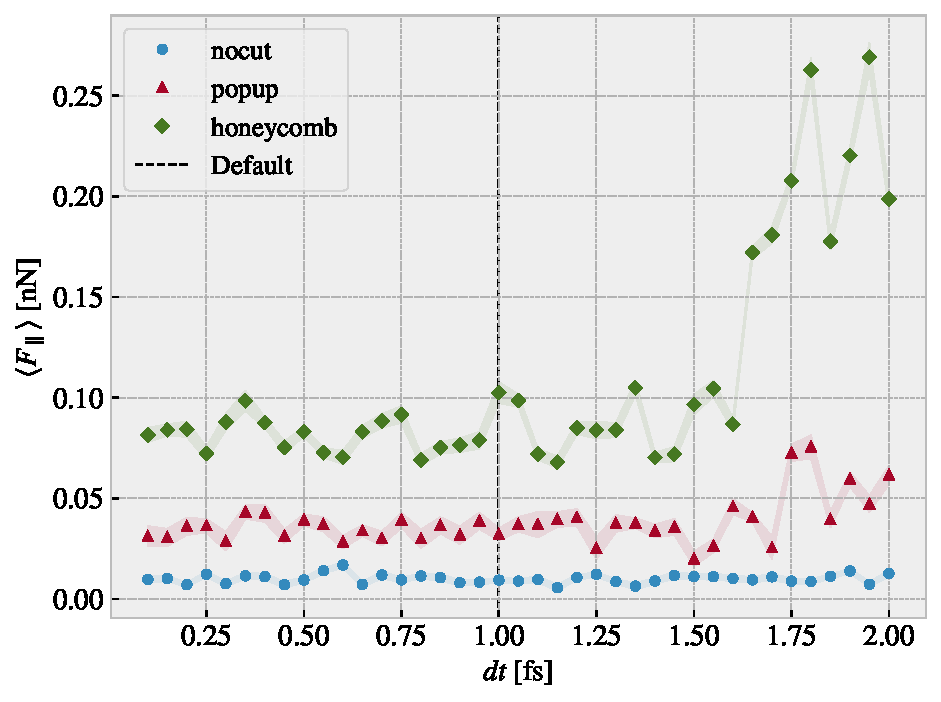
\includegraphics[width=\textwidth]{figures/baseline/variables_dt_mean_fixmove.pdf}
        \caption{}
        \label{fig:var_dt}
    \end{subfigure}
    \hfill
    \caption{Investigation of the friction dependencies to the selected parameters: temperature (a) sliding speed (b), spring constant (c) and timestep (d), the non-cut sheet, non-cut sheet, the Tetrahedron $(7,5,1)$, and the Honeycomb $(2,2,1,5)$ patterns. The dotted line denotes the default parameter choice and the shaded area denotesthe estimated ($\pm$) absolute error.}
    \label{fig:main_param}
\end{figure}

From the temperature investigation in~\cref{fig:var_temp} we find an increasing
kinetic friction with temperature for both the non-cut sheet and the Honeycomb
pattern. The Tetrahedron pattern shows both decreasing and increasing trends.
The general trend shows a convex curve in the range (30--480 K) with a minimum
around our default choice of \SI{300}{K}, but with rapid fluctuations at the
start (10--30 K) and end region (480--500 K). Similar fluctuations are also seen
from the Honeycomb pattern, although it shows an underlying increasing trend
throughout. When comparing the non-cut sheet and the Honeycomb pattern we
observe that the slope for the increasing trend is higher for the Honeycomb
pattern. From the predictions of the Prandtl–Tomlinson model and experimental results we expect to find a decrease in friction with increasing temperature. However, in similar \acrshort{MD}-based studies by Guerra et al.~\cite{Guerra_2010} they report that the frictional temperature dependence reverses at high sliding speed. They attribute this to the crossover from the diffusive to the ballistic regime taking place at a sliding speed of 1 to \SI{10}{m/s}. This agrees with our observations since we are using a sliding speed of \SI{20}{m/s}. In the absence of any clear suggestions from the results regarding an appropriate temperature, we take the common choice of using the room temperature \SI{300}{K}. The non-cut and Tetrahedon friction shows to be rather
stable around our temperature of choice, although we do see some significant fluctuations for the Honeycomb pattern in this range. However, we do not regard this as a critical feature.

From the sliding speed investigation in~\cref{fig:var_vel} we generally find
increasing friction with velocity. Due to the relatively high velocities used in
these simulations, we expect a viscous friction $F_k \propto v_{\text{sliding}}$
as reported by Guerra et al.~\cite{Guerra_2010} and predicted by the
Prandtl–Tomlinson model. In general, this aligns rather well with our results,
especially for the non-cut sheet. However, the Tetrahedron and Honeycomb sheets
seem to fall slightly into a sublinear relationship as it approaches higher
velocities. This behavior could potentially be attributed to velocity
saturation, a phenomenon predicted by the Prandtl-Tomlinson model without
considering the damping effect of the thermostat. On the other hand,
experimental results generally show a logarithmic increase in friction with
velocity, which may align better with the behavior observed for the Tetrahedron
pattern. Furthermore, we find that the Tetrahedron and Honeycomb patterns both
display indications of local fluctuations that could be attributed
to phonon resonance effects, as discussed in relation to the Frenkel-Kontorova
models. Our choice of a sliding speed at \SI{20}{m/s} mainly reflects a
consideration of computational cost, but the fact that no immediate resonance
fluctuations appear in the proximity of this value supports the choice further.  

From the investigation of the spring constant parameter in~\cref{fig:var_K} we observe a significant decrease in friction as the springs stiffen. This can be attributed to the transition from a stick-slip influenced regime to a smooth sliding regime as evidenced by the force traces in~\cref{fig:drag_Ff}. For soft springs the friction response is quite sensitive to the specific choice of spring constant which is especially seen for the non-cut sheet around $K = \SI{40}{N/m}$. Thus, in order to avoid this domain we settled for the infinitely stiff spring. This is also considered a more favorable option due to its ability to provide greater standardization of the simulations since it allows for a more controlled movement of the sheet.

Finally, we consider the numerical stability of the simulation result as we vary
the simulation timestep in~\cref{fig:var_dt}. The results indicate that the simulation is generally stable below a timestep of $\sim \SI{1.5}{fs}$, beyond which instability arises for the cut sheets (Tetrahedron and Honeycomb). This confirms that our choice of timestep is reasonable, but we do observe some fluctuations that are more pronounced for the cut sheets. These fluctuations imply that randomness plays a role in our simulations and that the cut sheets exhibit relatively higher instability compared to the non-cut sheet. Further investigation through varying the random seed for the initial velocity and thermostat could shed more light on this matter. In the meantime, we may consider these fluctuations as a sign that the uncertainty in our results is higher than our estimation from using the running mean and running \acrshort{std}. For the Honeycomb sheet, these fluctuations are on the order of $\pm \SI{0.017}{nN}$.



\subsection{Computational cost}
Our simulations are carried out on a CPU cluster made available by the University of Oslo. This allows us to run multiple simulations at once and with each simulation running in parallel on multiple CPU cores as well. When selecting the simulation parameters, we also need to keep in mind the computational cost. Given that the chosen parameters will be applied to multiple simulations, any increase in computational time will be multiplied by the number of intended simulations, which is roughly 10,000. The computational cost is especially dependent on the timestep and the sliding speed as this will affect the number of computations. As an extension of the analysis in~\cref{sec:main_params} we
report on the computational times associated with temperature, sliding speed,
spring constant and timestep. By retrieving the computational time used for the
parameter investigation in~\cref{fig:main_param} we get the timing shown in~\cref{fig:comp_cost}. Note that these timings are only based on a single simulation for each parameter as opposed to an average over multiple runs which is
necessary for more reliable data. 


\begin{figure}[H]
  \centering
  \begin{subfigure}[t]{0.49\textwidth}
      \centering
      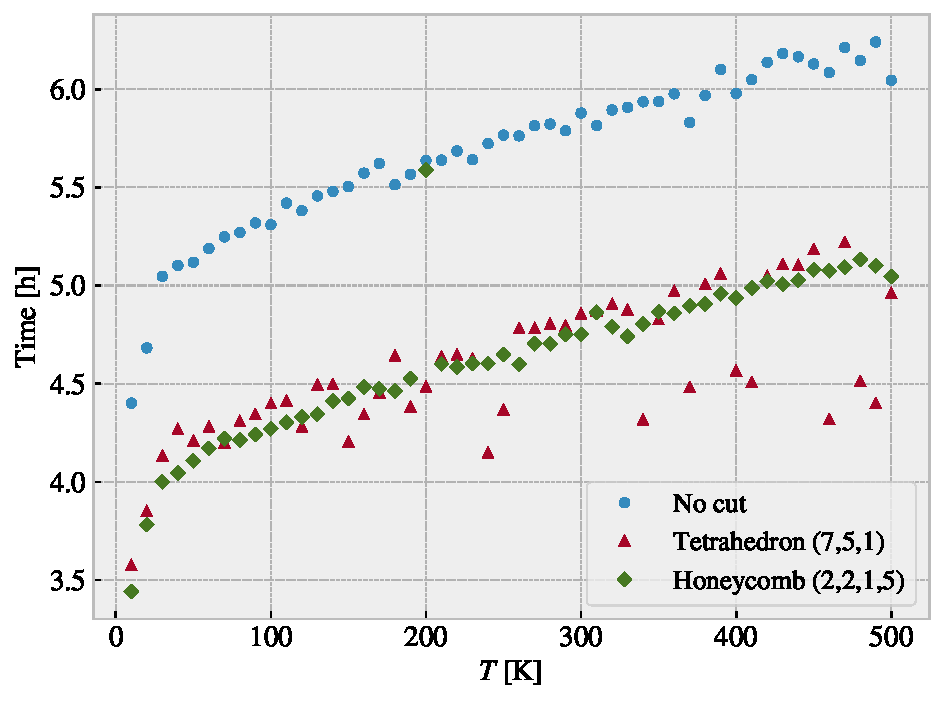
\includegraphics[width=\textwidth]{figures/baseline/comp_cost_temp.pdf}
      \caption{}
      \label{fig:comp_temp}
    \end{subfigure}
    \hfill
    \begin{subfigure}[t]{0.49\textwidth}
      \centering
      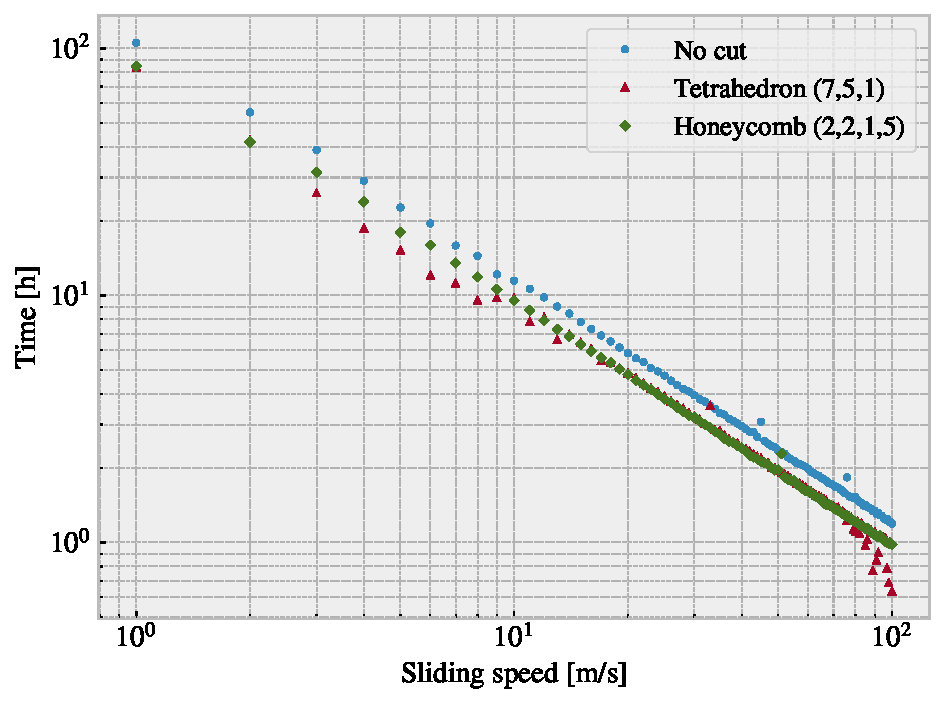
\includegraphics[width=\textwidth]{figures/baseline/comp_cost_vel.pdf}
      \caption{}
      \label{fig:comp_vel}
    \end{subfigure}
    \hfill
    \begin{subfigure}[t]{0.49\textwidth}
      \centering
      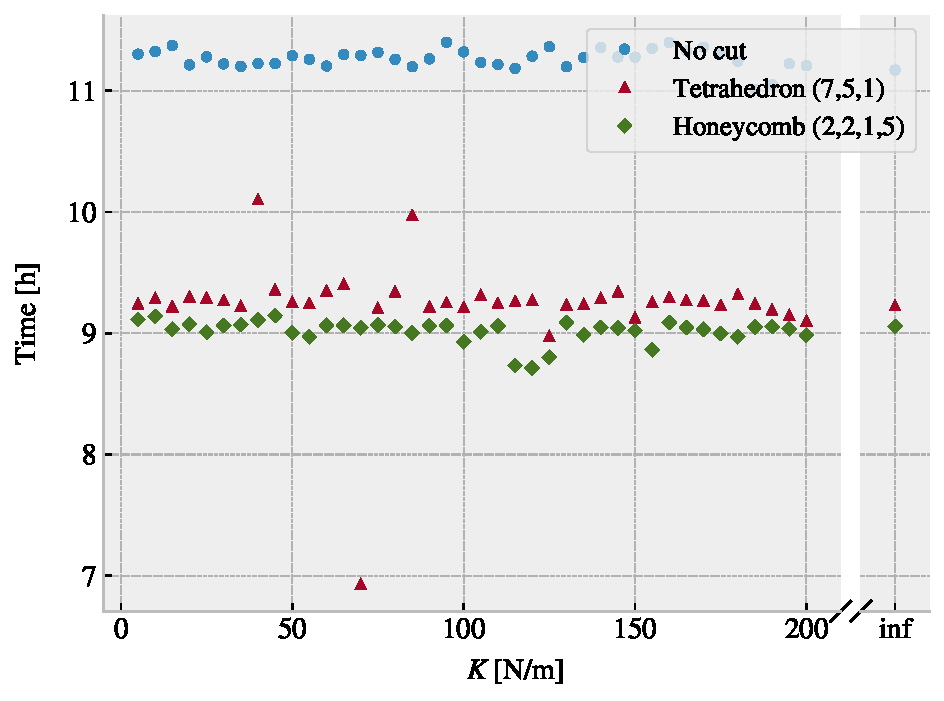
\includegraphics[width=\textwidth]{figures/baseline/comp_cost_K.pdf}
      \caption{}
      \label{fig:comp_K}
    \end{subfigure}
    \hfill
    \begin{subfigure}[t]{0.49\textwidth}
        \centering
        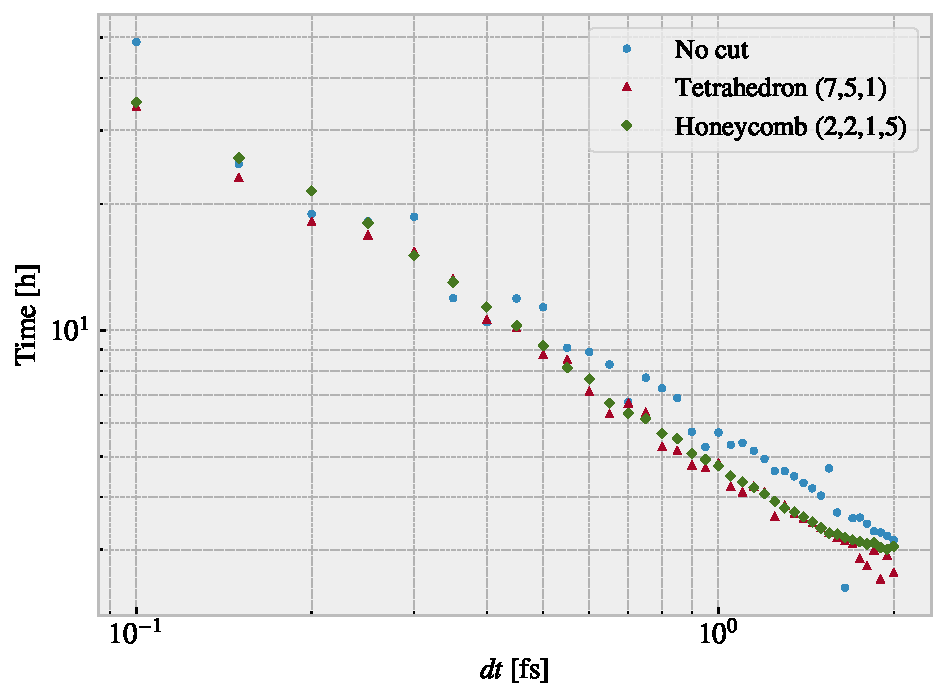
\includegraphics[width=\textwidth]{figures/baseline/comp_cost_dt.pdf}
        \caption{}
        \label{fig:comp_dt}
    \end{subfigure}
    \hfill
    \caption{The computational cost related to the parameter choice of temperature, sliding speed, spring
    constant and timestep, in terms of CPU hours running on 16 cores on the
    CPU cluster. The timing of the sliding speed is found to $t \propto
    v^{-0.977 \pm 0.005}$ while the timing for the timestep follows $t \propto \text{dt}^{-0.87\pm 0.02}$.}
    \label{fig:comp_cost}
\end{figure}

The computational time is governed by the number of timesteps in the simulation
and the time used per timestep. For a fixed sliding distance, the number of timesteps in the simulation is inversely proportional
to sliding speed and similar inversely proportional to timestep $dt$. From the
results in~\cref{fig:comp_cost} we find that the sliding speed obeys this
expectation rather well by $t \propto v^{-0.977 \pm 0.005}$. The timing did not increase as strongly as expected for the timestep, falling below the $1/dt$ relation with $t
\propto \text{dt}^{-0.87\pm 0.02}$. Moreover, we find that increasing
temperature also makes for an increased computation time. This can be attributed
to an increase in the computation time associated with the force calculations. The
rising temperature gives rise to more fluctuations in the system which might
yield more atoms within the force calculation cutoffs for each computation. This kind of consideration can also be attributed to the reason for the deviating timing for $dt$. Finally, for the spring parameter, we did not see any noticeable effect on timing.


In general, we have selected our simulation parameters: temperature, sliding speed, spring constant, and timestep, based on numerical stability
and computational cost. For the timestep, we found that a value of \SI{1}{fs},
commonly used in similar studies \cite{liu_high-speed_2014, zhu_study_2018},
produced stable results while higher values were prone to instabilities and
lower values were computationally expensive. The sliding speed was chosen primarily based on computational cost, with a default value of \SI{20}{m/s} being a reasonable compromise between computational efficiency and relatability to the lower values more commonly used in other studies. Although a lower sliding speed could lead to an interesting regime governed by stick-slip motion, it represents a factor of 20 increase in computational time. Since stick-slip motion is out of reach based on the chosen sliding speed, we found that using an infinitely stiff spring $K = \infty$ was the most reasonable option to ensure stable results. Finally, the temperature investigation did not provide much guidance for a specific choice, so we settled for the standard choice of room temperature $T = \SI{300}{K}$.



\section{Load and stretch dependencies}\label{sec:load_and_stretch}
So far, we have carried out a general analysis of the system behavior under the influence of various simulation parameters. This lays the foundation for the remaining study as we now shift our intention towards the friction dependence of strain and load.

\subsection{Pressure reference for normal load}
We consider a load range of 0.1--\SI{10}{nN} which coincides with the general investigated range in other \acrshort{MD} studies~\cite{li_evolving_2016, zhu_study_2018, zhu_study_2018}. In order to relate the magnitude of this load we provide a short calculation of the corresponding pressure. We will use the pressure underneath a stiletto-heeled shoe as a high-pressure reference from a macroscale perspective. The diameter of a stiletto-heeled
shoe can be less than \SI{1}{cm}~\cite{stiletto_1}, and hence an \SI{80}{kg} man\footnote{Yes, a man can certainly
wear stiletto heels.} standing on one stiletto heel, with all the weight on the heel, will generate a pressure
\begin{align*}
  P = \frac{F}{A} = \frac{mg}{r^2\pi} = \frac{\SI{80}{kg} \cdot \SI{9.8}{\frac{m}{s^2}}}{(\frac{\SI{e-2}{m}}{2})^2 \pi} = \SI{9.98}{MPa}.
\end{align*} 
The fact that the pressure under a stiletto heel can get this high, actually greater than the pressure under an elephant foot, is an interesting realization in itself that is often used in
introductory physics courses~\cite{stiletto_2}. Nonetheless, this serves as a reasonable upper bound for human executed pressure. With
a full sheet area of $\sim \SI{212}{nm^2}$ our load range of 0.1--\SI{10}{nN} corresponds to a pressure of 0.47--\SI{47}{MPa} which relates reasonably to our macroscale reference. This pressure might be incompatible with various industrial purposes, but with no specific application in mind, this serves as a decent reference point. Notice, that if we consider a human foot with the area \SI{113}{cm^2}~\cite{stiletto_3} the pressure drops to a mere \SI{70}{kPa} corresponding to only $\sim \SI{0.01}{nN}$.


\subsection{Strain dependency}\label{sec:stretch_dependency}
We consider the effects of stretching the sheet using the non-cut, Tetrahedron $(7,5,1)$ and Honeycomb $(2,2,1,5)$ sheet as used so far. For each configuration, we run a rupture test where the given sheet is strained under zero load, but still under the influence of adhesion from the substrate. The rupture strain is then recorded, and multiple new simulations are initiated with strain values between zero and the rupture strain. For the sampling of the strain values, we use uniformly spaced values between zero and the rupture strain. First, we aim to reproduce the contact investigation from~\cref{fig:contact_vs_stretch}. We quantify the relative contact as described in~\cref{sec:out-of-plane_buckling}, but we convert this into a single metric for a given simulation by considering the average of the last 50\% of the data points, similar
to what we have done for the mean friction. We also adopt a similar method for quantifying the error (see~\cref{sec:fric_metrics}). The results are shown
in~\cref{fig:contact_vs_stretch} where we observe a significant decrease in
relative contact with strain for the kirigami patterns. This agrees qualitatively with the non-loaded continuous strain simulations in~\cref{fig:contact_vs_stretch}. This result implies that the change in contact is not governed by a momentum effect during stretching, as each simulation now keeps a constant strain throughout. 
From an asperity theory point of view, the reduction in contact area is
theorized to induce a similar reduction in friction. However, when considering
the kinetic friction in~\cref{fig:multi_stretch_mean_fric} we find that this is
not the case. For the Tetrahedron and Honeycomb patterns, we find that the
friction initially increases with a decreasing contact area. Yet, these are not
simply inversely proportional as the friction force suddenly dips down and up
again, in the strain range of 0.08--0.11 for the Tetrahedron and 0.73--1.05 for
the Honeycomb pattern. When considering the non-cut sheet, we find that both the
contact area and friction remain seemingly unaffected by strain. This indicates
that the contact area is not a dominating mechanism for friction in our system,
although the non-linear friction-strain curve might be correlated with a
decrease in contact area through an underlying mechanism related to the out-of-plane buckling. This can be supported
by the fact that the contact-strain and friction-strain curves for the Honeycomb
pattern both show signs of a discontinuous jump around a strain of 0.32. Since
the non-cut sheet exhibits a flat friction-strain profile we cannot attribute
the behavior to an increased tension either. Zhang et
al.~\cite{zhang_tuning_2019} reported that the friction for a graphene sheet
decreases with tension which qualitatively contradicts our observation and
supports that tension is not a governing mechanism. Instead,
we might attribute the results to a commensurability effect or perhaps a change in the
structural stiffness which is reported as an important feature by
\cite{Kim_2012}. 

We notice that the initial friction value of the non-strained sheet varies among different configurations, with the non-cut sheet exhibiting the lowest initial friction value ($\sim \SI{7e-4}{nN}$), the Tetrahedron sheet having a slightly higher value ($\sim \SI{0.03}{nN}$), and the Honeycomb sheet exhibiting the highest ($\sim \SI{0.07}{nN}$). This is more clearly shown in the parameter investigation in~\cref{fig:main_param}. The magnitude of this effect is generally one order of magnitude lower than the strain-induced friction effect. We notice also that the two orders of magnitude increase in normal load did not
make a significant difference in the results. The estimated absolute error
marked by a shaded area in~\cref{fig:multi_stretch_mean_fric} were fairly low
for both friction on the order \SI{e-3}{nN} and relative contact on the order of
\num{e-4}.


\begin{figure}[H]
  \centering
  \begin{subfigure}[t]{\textwidth}
      \centering
      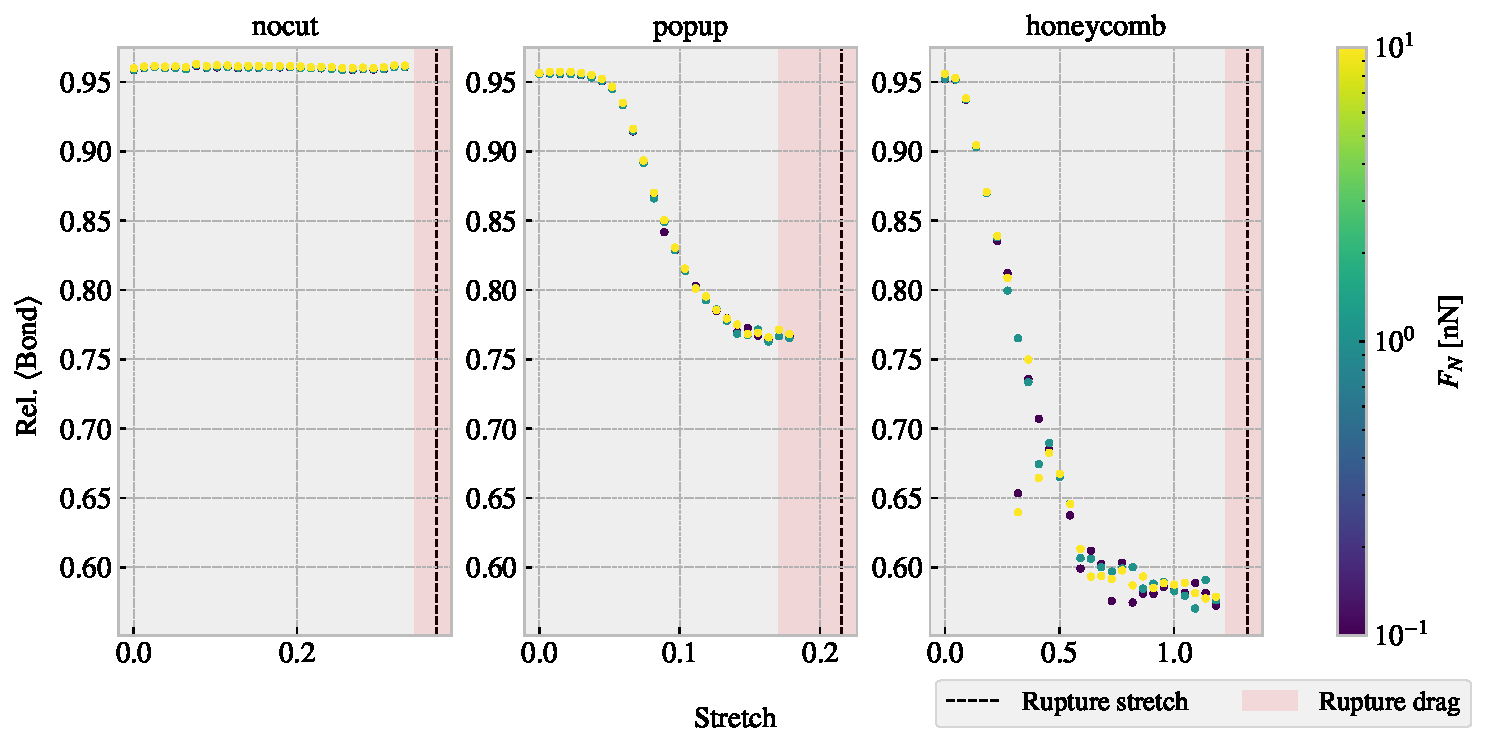
\includegraphics[width=\textwidth]{figures/baseline/multi_stretch_area_compare.pdf}
      \caption{}
      \label{fig:fig:multi_stretch_contact}
  \end{subfigure}
  \hfill
  \begin{subfigure}[t]{\textwidth}
      \centering
      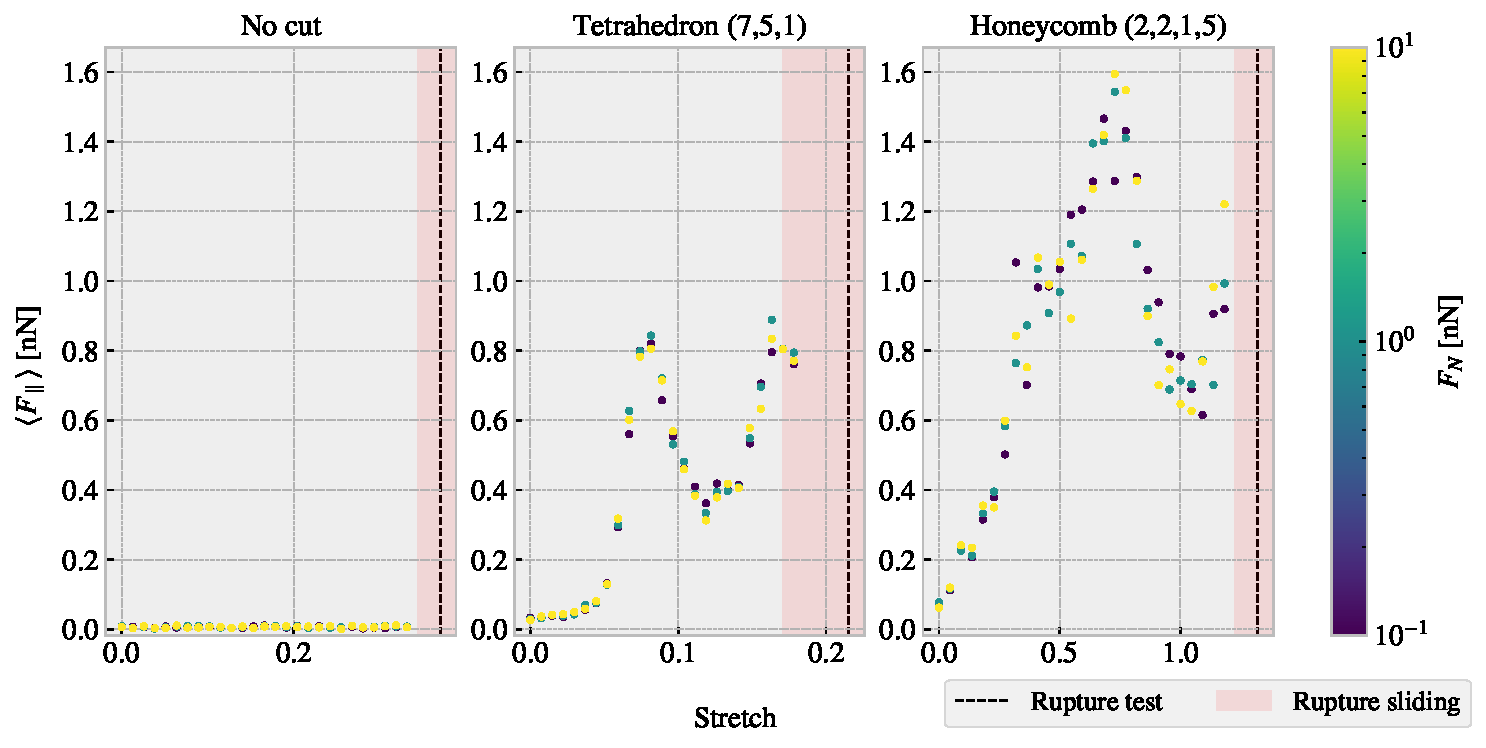
\includegraphics[width=\textwidth]{figures/baseline/multi_stretch_mean_compare.pdf}
      \caption{}
      \label{fig:multi_stretch_mean_fric}
  \end{subfigure}
  \hfill
     \caption{Mean relative contact and mean friction for multiple simulations,
     consisting of 30 strain values uniformly spaced 0 and the rupture strain in combination with loads 0.1, 1 and
     \SI{10}{nN}, for each of the configurations: non-cut, Tetrahedron $(7,5,1)$
     and Honeycomb $(2,2,1,5)$. The average is taken over the last half of the
     sliding phase, and the shaded area connecting the dots linearly indicates
     the absolute error. The red shade denotes the strain range where ruptures
     occurred during sliding while the black-dotted line represents the rupture
     point in the non-loaded rupture test. (a) The average relative contact
     defined as the relative number of atoms within a contact threshold of
     \SI{4}{\text{Å}} to the substrate. The absolute error is generally on the
     order \num{e-4}. (b) The average mean friction force parallel to the
     sliding direction. The absolute error for the mean friction is on the order
     \SI{e-3}{nN}.}
     \label{fig:multi_stretch}
\end{figure}

By considering the increase in friction from zero strain towards the first peak
of the friction-strain curve we find that the Tetrahedron pattern exhibits a
relative friction increase of $\sim 27.7$ while the Honeycomb pattern exhibits a
relative increase of $\sim 22.4$. This is in itself a remarkable result, but
considering that the friction drops almost as dramatically afterward is even more unexpected. For the Tetrahedron pattern, the friction drops by
$\sim \SI{0.51}{nN}$ during an increased strain $\Delta \varepsilon \sim 0.04$
while for the Honeycomb pattern the friction drops $\sim\SI{0.98}{nN}$ during a strain increase of $\Delta \varepsilon \sim 0.36$. These results are promising for the aim of demonstrating a negative friction coefficient for a system with coupled load and strain. We will discuss this further at the end of this chapter in~\cref{sec:neg_prospects}.



\subsection{Load dependency}\label{sec:load_dependency}
From the investigation of the strain dependency we saw that increasing the normal load from 0.1 to \SI{10}{nN} did not make a considerable impact on the friction in comparison to the effect associated with strain. One special feature of our system is that we only apply load to the pull blocks, and thus one might suspect this to be of importance. Therefore, we investigate the friction under varying loads for a non-cut sheet comparing the case of loading the pull block against a  uniform loading of the sheet as shown in~\cref{fig:load_dist}. Both load distributions show a seemingly non-dependent relationship between friction and load considering the size of our estimated error. Thus, we do not find any indications that the uniform loading changes the qualitative behavior of our system.

\begin{figure}[H]
  \centering
  \begin{subfigure}[t]{0.49\textwidth}
      \centering
      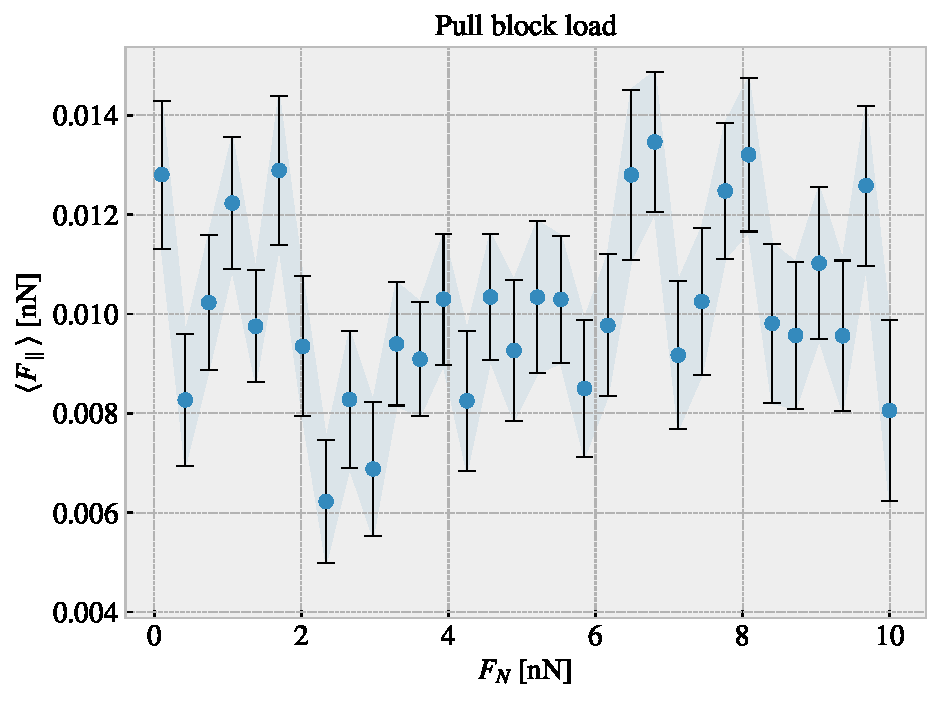
\includegraphics[width=\textwidth]{figures/baseline/load_dist_a.pdf}
      \caption{}
      \label{fig:load_dist_a}
  \end{subfigure}
  \hfill
  \begin{subfigure}[t]{0.49\textwidth}
      \centering
      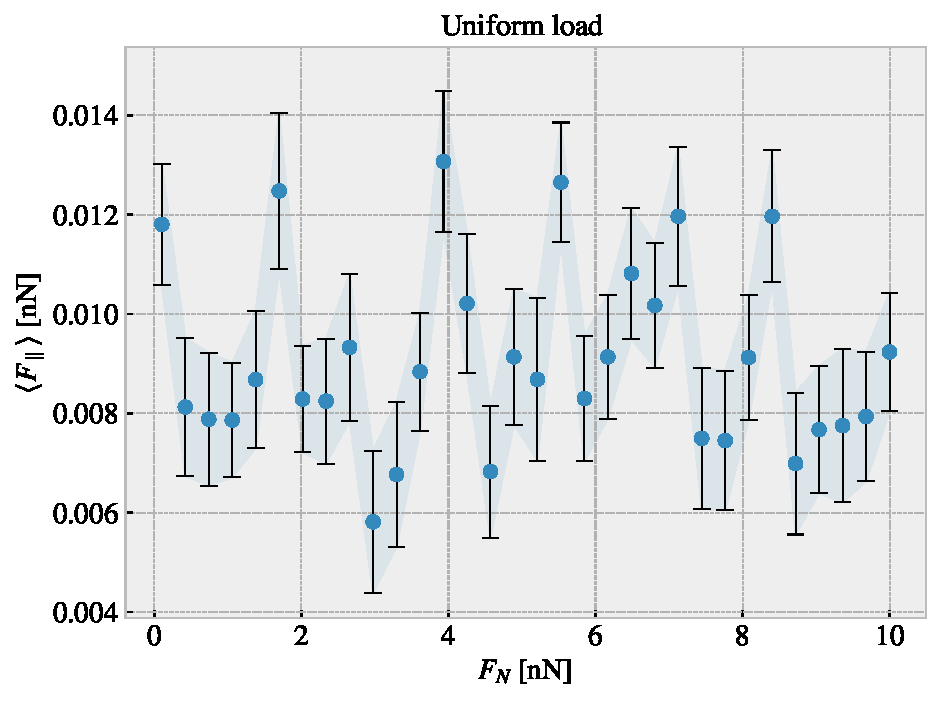
\includegraphics[width=\textwidth]{figures/baseline/load_dist_b.pdf}
      \caption{}
      \label{fig:load_dist_b}
  \end{subfigure}
  \hfill
     \caption{Multiple simulations of a non-cut sheet under various uniformly sampled load values $F_N \in [0.1, 10]$ nN for two different variations of loading distribution. The shading and the error bars denotes the absolute error. (a) The loading is applied to the pull blocks. (b) The loading is applied uniformly to the full sheet. }
     \label{fig:load_dist}
\end{figure}

To examine the relationship between friction and normal load as the Kirigami patterns undergo strain, we conduct additional simulations with a logarithmically increasing normal load in the range of 0.1 to \SI{100}{nN}. This is done for a selected subset of strain stages from~\cref{fig:multi_stretch_mean_fric}, with 30 load data points for each strain. We monitor the relative contact as well. The results are shown in~\cref{fig:load_dependency}. Upon varying the normal load over three orders of magnitude, we notice a small increase in friction with load for all Kirigami patterns. However, this effect is more pronounced for the non-cut sheet as the friction axis shows a narrower range for this pattern. 

It should be noted that due to the logarithmic scale of the load axis, any apparent linear trends in the figure is actually sublinear. However, as the normal load approaches \SI{100}{nN}, there is some indication of an increase in friction that is more reminiscent of a linear relationship. Nevertheless, it is difficult to draw firm conclusions as the change in friction is relatively small compared to the level of noise in the data. We find an increasing contact area with load, for which the increase is 

%
%
% Working here
%
%

. However the increase from \SI{0.1}{nN} to \SI{}


We generally find that the contact area increases with load which is somewhat expected due to the increased pressure on the sheet. However, the change in contact area is relatively low and thus it is difficult to draw any further conlusion to the relationship between friction and contact area.  



Note that we omitted the error bars for visual purposes but the absolute erros for both the relative contact and friction are on the same order of magnitude as shown in~\cref{fig:multi_stretch} and ~\cref{fig:load_dist}.


\begin{figure}[H]
  \centering
  \begin{subfigure}[t]{\textwidth}
      \centering
      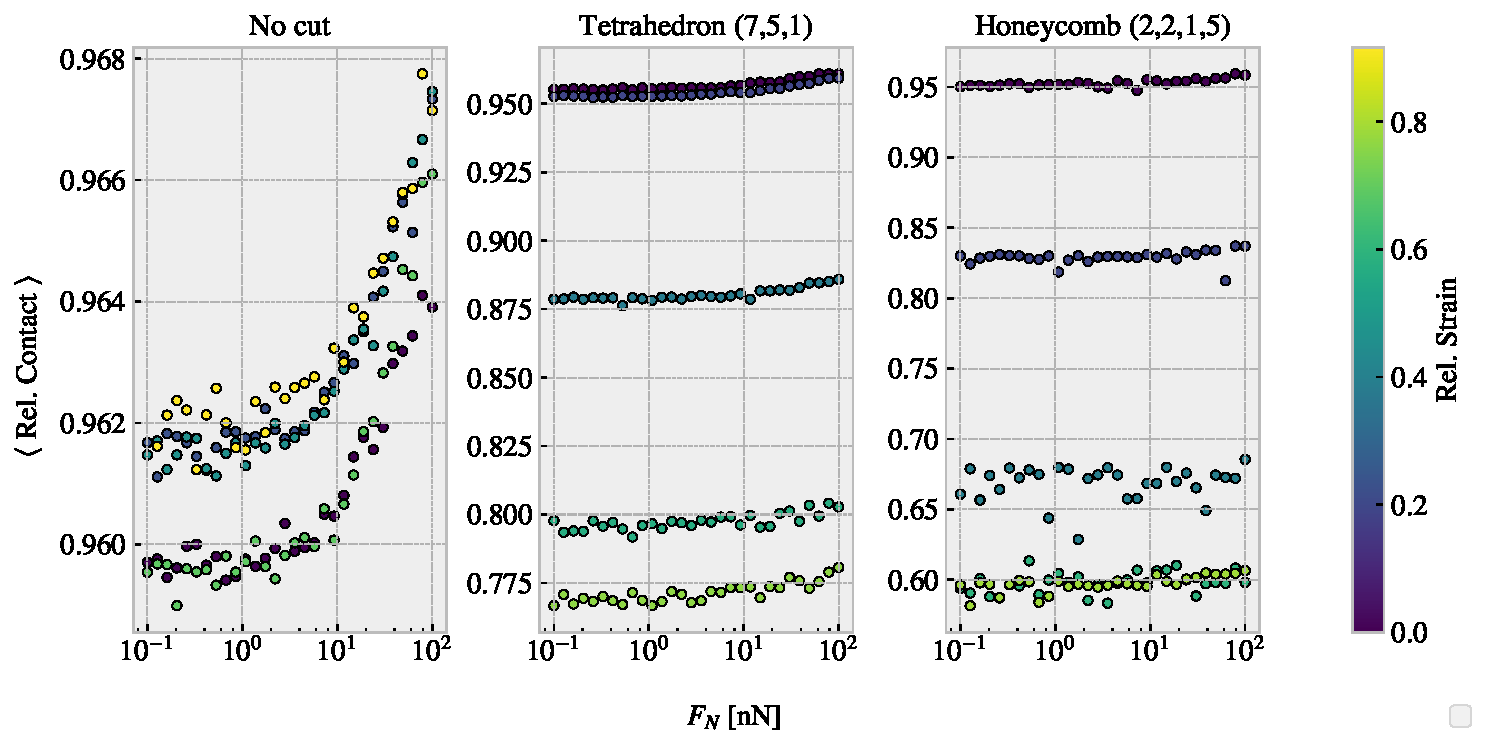
\includegraphics[width=\textwidth]{figures/baseline/multi_FN_contact_compare.pdf}
      \caption{}
      \label{fig:fig:multi_load_contact}
  \end{subfigure}
  \hfill
  \begin{subfigure}[t]{\textwidth}
      \centering
      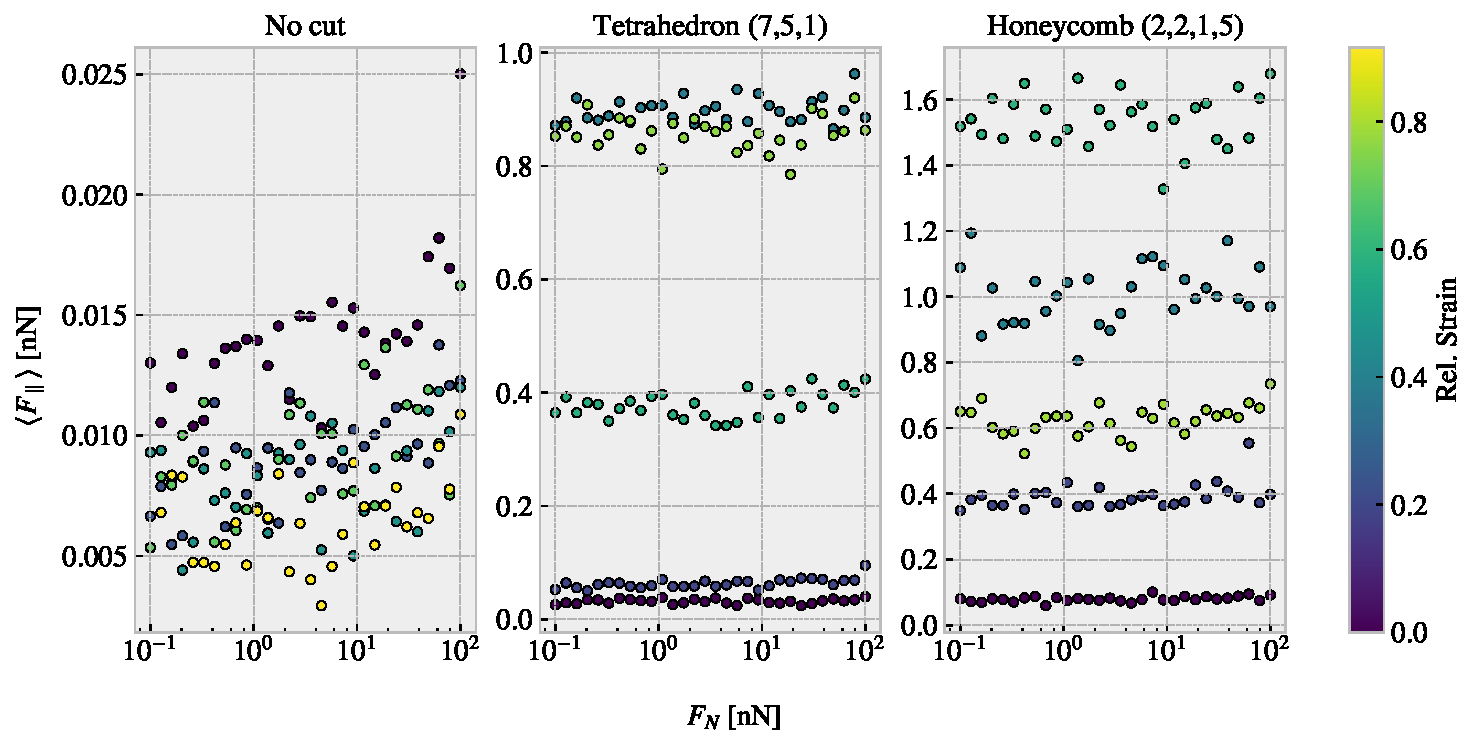
\includegraphics[width=\textwidth]{figures/baseline/multi_FN_mean_compare.pdf}
      \caption{}
      \label{fig:multi_load_fric}
  \end{subfigure}
  \hfill
     \caption{Mean relative contact and mean friction for multiple simulations, consisting of 30 logarithmically spaced load values in the range 0.1--\SI{100}{nN} for the non-cut, Tetrahedron $(7,5,1)$ and Honeycomb $(2,2,1,5)$ sheet respectively, at different strain stages relative to their rupture strains. (a) The average relative contact. (b) The average mean friction. We omitted the indication of the absolute errors as they were similarly low as seen in~\cref{fig:multi_stretch}.}
     \label{fig:multi_load}
\end{figure}

%
%
%
%
%
%


From the friction measurements in~\cref{fig:multi_load_fric} we see that the
non-cut sheet generally produces a friction force in the order of 0.005--\SI{0.0025}{nN} throughout the 0.1--\SI{100}{nN} load range. Using a ratio based friction coefficient definition \cref{eq:mu_def1}, $\mu_1 = F_{\text{fric}}/{F_N}$, this would lead to a coefficient roughly in the range
\begin{align*}
  &\mu_1,  \ \text{\cref{eq:mu_def1}:}& &\text{No cut}\sim [\num{e-4}, 0.13],&  &\text{Tetrahedron}\sim [\num{4e-4},8.7],& &\text{Honeycomb}\sim [\num{9e-4}, 15.2].&
\end{align*}
However, these values mainly reflect the poorness of this definition, as we find the values to diverge at low load and decrease towards high load due to the lacking linear relationship and an offset in the load curve corresponding to a finite friction at zero load. This offset is drastically enhanced for the Kirigami patterns under strain. Due to the small changes in friction compared to the noise in the data, it is not sensible to calculate the slope $dF_{\text{fric}}/dF_N$ as a function of load. Nonetheless, if we force a linear fit for the whole range and use the second definition \cref{eq:mu_def2} as $\langle \mu_2 \rangle = \Delta F_{\text{fric}}/\Delta F_N$, we get average coefficients in the range
\begin{align*}
  &\mu_2,  \ \text{\cref{eq:mu_def2}:}& &\text{No cut} \sim [4, 9]\times \num{e-5},&  &\text{Tetrahedron} \sim 5\times[\num{e-5}, \num{e-4}],& &\text{Honeycomb} \sim [1,9]\times \num{e-4},&
\end{align*}
depending on the strain values. These numbers should be interpreted cautiously,
but we can take it as a rough estimate of the friction coefficient being on
the order \num{e-4}--\num{e-5}. This relates to the finding by
\cite{DIENWIEBEL2005197} who reported a seemingly non-existing relationship
between friction and normal load with change in friction that corresponds to friction coefficients in the range \num{e-3}--\num{e-4} when using the slope definition \cref{eq:mu_def2}. This supports the idea that the graphene sheet does in fact exhibit superlubric behavior in these conditions. Moreover, the fact that the increase with load is relatively unaffected by the stretching points to the fact that the strain-induced effect mainly shifts the load curve towards higher friction but does not significantly alter its slope. 


\subsection{Prospects of a negative friction coefficient}\label{sec:neg_prospects}

Considering the results from~\cref{sec:stretch_dependency} and~\cref{sec:load_dependency} we find that strain-induced friction effects, on the order of $/SI{1}{nN}$, are generally dominating in comparison to load-induced effects on the order of \SI{0.01}{nN} given a load range of \SI{e2}{nN}. This is promising for the idea of achieving a negative friction coefficient for a nanomachine system that couples load and strain. By applying load on the nanomachine we would increase both the load and the strain on the sheet simultaneously. However, since the friction dependency to strain dominates in comparison to load effects such a system can be designed entirely by considering the strain dependency. The friction coefficient is by our definition (\cref{eq:mu_def2}) given as the slope of the friction $F_f$ vs.\ normal force $F_N$ curve. Hence, for two points $\{(F_{N,1}, F_{f,1}), (F_{N,2}, F_{f,2})\}$, $F_{N,1} < F_{N,2}$ we can evaluate the associated friction coefficient $\mu_{1,2}$ as 
\begin{align*}
  \mu_{1,2} = \frac{F_{f,2} - F_{f,1}}{F_{N,2} - F_{N,1}} = \frac{\Delta F_f}{\Delta F_N}.
\end{align*}
If we neglect load effects $F_f(F_N, \varepsilon) \sim F_f(\varepsilon)$ and consider a coupling $\varepsilon = R F_N$ with linear coupling ratio $R$ we get 
\begin{align}
  \mu_{1,2}(\varepsilon_1, \varepsilon_2) = \frac{\Delta F_{f}(\varepsilon_1, \varepsilon_2)}{\frac{1}{R}(\varepsilon_2 - \varepsilon_1)} = R\frac{\Delta F_{f}(\varepsilon_1, \varepsilon_2)}{\Delta \varepsilon}.
  \label{eq:mu_strain}
\end{align}
When considering the ratios found for the reduction in friction with strain for the Tetrahedron and Honeycomb patterns in~\cref{sec:stretch_dependency} we find the corresponding coupled system friction coefficients to be 
\begin{align}
  &\text{Tetrahedron:} \quad R\frac{-\SI{0.51}{nN}}{0.04} = -R\cdot\SI{12.75}{nN},& &\text{Honeycomb:} \quad R\frac{-\SI{0.98}{nN}}{0.36} = -R\cdot\SI{2.72}{nN}&
  \label{eq:pilot_study_mu_estimate}
\end{align}
This showcases that we might be able to utilize the strain effect to achieve a negative friction for the system of coupled strain and load







